\documentclass[]{article}
\usepackage{lmodern}
\usepackage{amssymb,amsmath}
\usepackage{ifxetex,ifluatex}
\usepackage{fixltx2e} % provides \textsubscript
\ifnum 0\ifxetex 1\fi\ifluatex 1\fi=0 % if pdftex
  \usepackage[T1]{fontenc}
  \usepackage[utf8]{inputenc}
\else % if luatex or xelatex
  \ifxetex
    \usepackage{mathspec}
  \else
    \usepackage{fontspec}
  \fi
  \defaultfontfeatures{Ligatures=TeX,Scale=MatchLowercase}
\fi
% use upquote if available, for straight quotes in verbatim environments
\IfFileExists{upquote.sty}{\usepackage{upquote}}{}
% use microtype if available
\IfFileExists{microtype.sty}{%
\usepackage{microtype}
\UseMicrotypeSet[protrusion]{basicmath} % disable protrusion for tt fonts
}{}
\usepackage[margin=1in]{geometry}
\usepackage{hyperref}
\hypersetup{unicode=true,
            pdftitle={Considerações sobre o impacto do valor do desvio-padrão},
            pdfauthor={Luiz Fernando Palin Droubi},
            pdfborder={0 0 0},
            breaklinks=true}
\urlstyle{same}  % don't use monospace font for urls
\usepackage{color}
\usepackage{fancyvrb}
\newcommand{\VerbBar}{|}
\newcommand{\VERB}{\Verb[commandchars=\\\{\}]}
\DefineVerbatimEnvironment{Highlighting}{Verbatim}{commandchars=\\\{\}}
% Add ',fontsize=\small' for more characters per line
\usepackage{framed}
\definecolor{shadecolor}{RGB}{248,248,248}
\newenvironment{Shaded}{\begin{snugshade}}{\end{snugshade}}
\newcommand{\KeywordTok}[1]{\textcolor[rgb]{0.13,0.29,0.53}{\textbf{#1}}}
\newcommand{\DataTypeTok}[1]{\textcolor[rgb]{0.13,0.29,0.53}{#1}}
\newcommand{\DecValTok}[1]{\textcolor[rgb]{0.00,0.00,0.81}{#1}}
\newcommand{\BaseNTok}[1]{\textcolor[rgb]{0.00,0.00,0.81}{#1}}
\newcommand{\FloatTok}[1]{\textcolor[rgb]{0.00,0.00,0.81}{#1}}
\newcommand{\ConstantTok}[1]{\textcolor[rgb]{0.00,0.00,0.00}{#1}}
\newcommand{\CharTok}[1]{\textcolor[rgb]{0.31,0.60,0.02}{#1}}
\newcommand{\SpecialCharTok}[1]{\textcolor[rgb]{0.00,0.00,0.00}{#1}}
\newcommand{\StringTok}[1]{\textcolor[rgb]{0.31,0.60,0.02}{#1}}
\newcommand{\VerbatimStringTok}[1]{\textcolor[rgb]{0.31,0.60,0.02}{#1}}
\newcommand{\SpecialStringTok}[1]{\textcolor[rgb]{0.31,0.60,0.02}{#1}}
\newcommand{\ImportTok}[1]{#1}
\newcommand{\CommentTok}[1]{\textcolor[rgb]{0.56,0.35,0.01}{\textit{#1}}}
\newcommand{\DocumentationTok}[1]{\textcolor[rgb]{0.56,0.35,0.01}{\textbf{\textit{#1}}}}
\newcommand{\AnnotationTok}[1]{\textcolor[rgb]{0.56,0.35,0.01}{\textbf{\textit{#1}}}}
\newcommand{\CommentVarTok}[1]{\textcolor[rgb]{0.56,0.35,0.01}{\textbf{\textit{#1}}}}
\newcommand{\OtherTok}[1]{\textcolor[rgb]{0.56,0.35,0.01}{#1}}
\newcommand{\FunctionTok}[1]{\textcolor[rgb]{0.00,0.00,0.00}{#1}}
\newcommand{\VariableTok}[1]{\textcolor[rgb]{0.00,0.00,0.00}{#1}}
\newcommand{\ControlFlowTok}[1]{\textcolor[rgb]{0.13,0.29,0.53}{\textbf{#1}}}
\newcommand{\OperatorTok}[1]{\textcolor[rgb]{0.81,0.36,0.00}{\textbf{#1}}}
\newcommand{\BuiltInTok}[1]{#1}
\newcommand{\ExtensionTok}[1]{#1}
\newcommand{\PreprocessorTok}[1]{\textcolor[rgb]{0.56,0.35,0.01}{\textit{#1}}}
\newcommand{\AttributeTok}[1]{\textcolor[rgb]{0.77,0.63,0.00}{#1}}
\newcommand{\RegionMarkerTok}[1]{#1}
\newcommand{\InformationTok}[1]{\textcolor[rgb]{0.56,0.35,0.01}{\textbf{\textit{#1}}}}
\newcommand{\WarningTok}[1]{\textcolor[rgb]{0.56,0.35,0.01}{\textbf{\textit{#1}}}}
\newcommand{\AlertTok}[1]{\textcolor[rgb]{0.94,0.16,0.16}{#1}}
\newcommand{\ErrorTok}[1]{\textcolor[rgb]{0.64,0.00,0.00}{\textbf{#1}}}
\newcommand{\NormalTok}[1]{#1}
\usepackage{graphicx,grffile}
\makeatletter
\def\maxwidth{\ifdim\Gin@nat@width>\linewidth\linewidth\else\Gin@nat@width\fi}
\def\maxheight{\ifdim\Gin@nat@height>\textheight\textheight\else\Gin@nat@height\fi}
\makeatother
% Scale images if necessary, so that they will not overflow the page
% margins by default, and it is still possible to overwrite the defaults
% using explicit options in \includegraphics[width, height, ...]{}
\setkeys{Gin}{width=\maxwidth,height=\maxheight,keepaspectratio}
\IfFileExists{parskip.sty}{%
\usepackage{parskip}
}{% else
\setlength{\parindent}{0pt}
\setlength{\parskip}{6pt plus 2pt minus 1pt}
}
\setlength{\emergencystretch}{3em}  % prevent overfull lines
\providecommand{\tightlist}{%
  \setlength{\itemsep}{0pt}\setlength{\parskip}{0pt}}
\setcounter{secnumdepth}{5}
% Redefines (sub)paragraphs to behave more like sections
\ifx\paragraph\undefined\else
\let\oldparagraph\paragraph
\renewcommand{\paragraph}[1]{\oldparagraph{#1}\mbox{}}
\fi
\ifx\subparagraph\undefined\else
\let\oldsubparagraph\subparagraph
\renewcommand{\subparagraph}[1]{\oldsubparagraph{#1}\mbox{}}
\fi

%%% Use protect on footnotes to avoid problems with footnotes in titles
\let\rmarkdownfootnote\footnote%
\def\footnote{\protect\rmarkdownfootnote}

%%% Change title format to be more compact
\usepackage{titling}

% Create subtitle command for use in maketitle
\newcommand{\subtitle}[1]{
  \posttitle{
    \begin{center}\large#1\end{center}
    }
}

\setlength{\droptitle}{-2em}

  \title{Considerações sobre o impacto do valor do desvio-padrão}
    \pretitle{\vspace{\droptitle}\centering\huge}
  \posttitle{\par}
  \subtitle{nas amostras de distribuição lognormal}
  \author{Luiz Fernando Palin Droubi}
    \preauthor{\centering\large\emph}
  \postauthor{\par}
      \predate{\centering\large\emph}
  \postdate{\par}
    \date{18 de outubro de 2018}


\begin{document}
\maketitle

\section{INTRODUÇÃO}\label{introducao}

Segundo Limpert (LIMPERT et al., 2001, p. 346), distribuições lognormais
de diversas ciências tem, em geral, valores de \(s^*\) variando de 1,1 a
33 (na escala natural, entre 0,095 e 3,497), sendo que o mais comum é
que estes valores estejam entre 1,4 e 3 (0,336 \(\leq s \leq\) 1,099).

Na Engenharia de Avaliações, temos:

\begin{Shaded}
\begin{Highlighting}[]
\KeywordTok{data}\NormalTok{(centro_}\DecValTok{2015}\NormalTok{)}
\NormalTok{dados <-}\StringTok{ }\NormalTok{centro_}\DecValTok{2015}\OperatorTok{@}\NormalTok{data}
\NormalTok{dados <-}\StringTok{ }\NormalTok{dados[}\KeywordTok{complete.cases}\NormalTok{(dados), ]}
\NormalTok{x <-}\StringTok{ }\KeywordTok{exp}\NormalTok{(}\KeywordTok{mean}\NormalTok{(}\KeywordTok{log}\NormalTok{(dados}\OperatorTok{$}\NormalTok{valor)))}
\NormalTok{s <-}\KeywordTok{exp}\NormalTok{(}\KeywordTok{sqrt}\NormalTok{(}\KeywordTok{sum}\NormalTok{(}\KeywordTok{log}\NormalTok{(dados}\OperatorTok{$}\NormalTok{valor}\OperatorTok{/}\NormalTok{x)}\OperatorTok{^}\DecValTok{2}\NormalTok{)}\OperatorTok{/}\KeywordTok{length}\NormalTok{(dados}\OperatorTok{$}\NormalTok{valor)))}
\NormalTok{f1 <-}\StringTok{ }\KeywordTok{fitdist}\NormalTok{(dados}\OperatorTok{$}\NormalTok{valor, }\StringTok{"lnorm"}\NormalTok{, }\DataTypeTok{method =} \StringTok{"mle"}\NormalTok{)}
\end{Highlighting}
\end{Shaded}

\begin{itemize}
\tightlist
\item
  Hochheim (HOCHHEIM, 2015, p. 21): \(s^* =\) 1,851.
\end{itemize}

\section{EXEMPLO 1}\label{exemplo-1}

\subsection{GERAÇÃO DE DADOS
RANDÔMICOS}\label{geracao-de-dados-randomicos}

\begin{Shaded}
\begin{Highlighting}[]
\KeywordTok{set.seed}\NormalTok{(}\DecValTok{1}\NormalTok{)}
\NormalTok{x <-}\StringTok{ }\KeywordTok{seq}\NormalTok{(}\DecValTok{1}\NormalTok{, }\DecValTok{100}\NormalTok{, }\FloatTok{0.5}\NormalTok{)}
\NormalTok{y <-}\StringTok{ }\KeywordTok{exp}\NormalTok{(x}\OperatorTok{/}\DecValTok{25} \OperatorTok{+}\StringTok{ }\KeywordTok{rnorm}\NormalTok{(}\DecValTok{199}\NormalTok{, }\DataTypeTok{sd =}\NormalTok{ .}\DecValTok{1}\NormalTok{)) }
\end{Highlighting}
\end{Shaded}

\subsection{GRÁFICOS}\label{graficos}

\begin{Shaded}
\begin{Highlighting}[]
\KeywordTok{plot}\NormalTok{(}\KeywordTok{log}\NormalTok{(y) }\OperatorTok{~}\StringTok{ }\NormalTok{x)}
\end{Highlighting}
\end{Shaded}

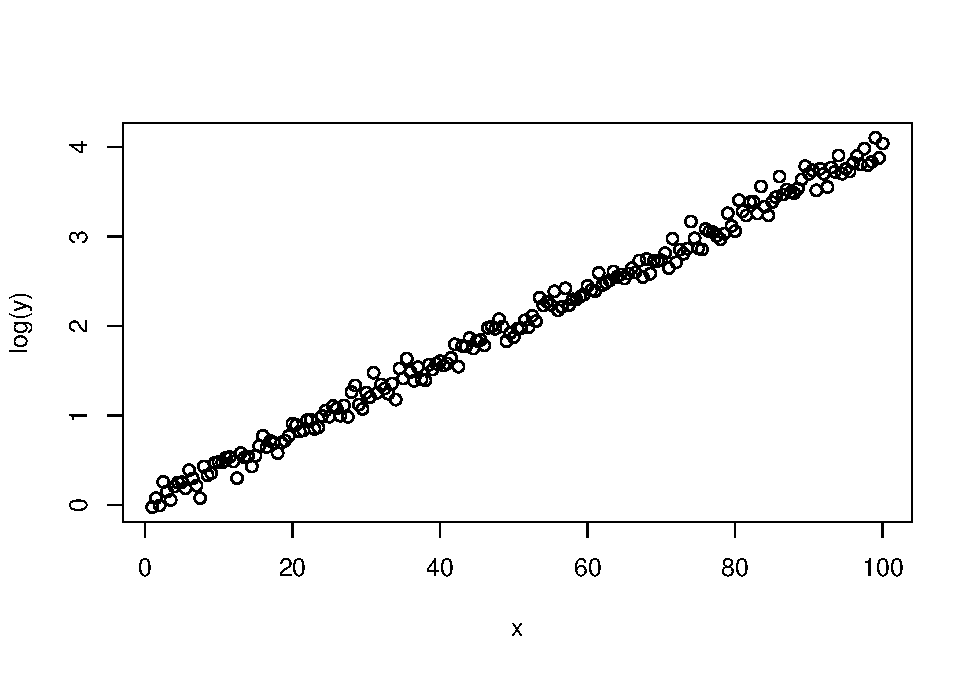
\includegraphics{Impacto_sigma_files/figure-latex/unnamed-chunk-3-1.pdf}

\begin{Shaded}
\begin{Highlighting}[]
\KeywordTok{histogram}\NormalTok{(y)}
\KeywordTok{plotDist}\NormalTok{(}\StringTok{"lnorm"}\NormalTok{, }
         \DataTypeTok{meanlog =} \KeywordTok{mean}\NormalTok{(}\KeywordTok{log}\NormalTok{(y), }\DataTypeTok{na.rm =} \OtherTok{TRUE}\NormalTok{),}
         \DataTypeTok{sdlog =} \KeywordTok{sd}\NormalTok{(}\KeywordTok{log}\NormalTok{(y), }\DataTypeTok{na.rm =} \OtherTok{TRUE}\NormalTok{), }
         \DataTypeTok{add =} \OtherTok{TRUE}\NormalTok{)}
\end{Highlighting}
\end{Shaded}

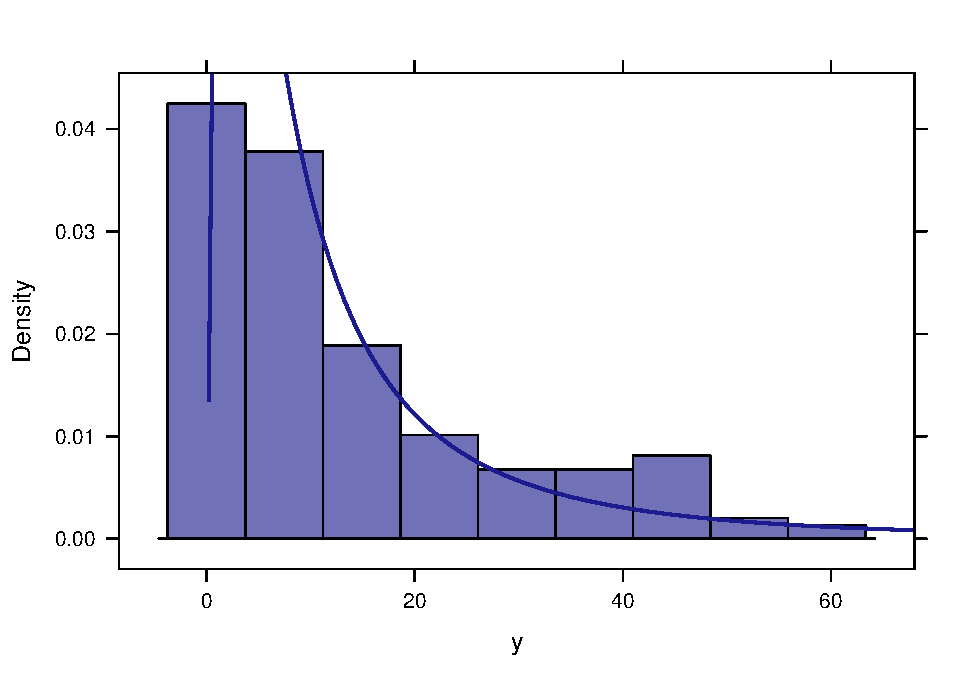
\includegraphics{Impacto_sigma_files/figure-latex/unnamed-chunk-4-1.pdf}

\subsection{MODELO}\label{modelo}

\begin{Shaded}
\begin{Highlighting}[]
\NormalTok{fit <-}\StringTok{ }\KeywordTok{lm}\NormalTok{(}\KeywordTok{log}\NormalTok{(y) }\OperatorTok{~}\StringTok{ }\NormalTok{x)}
\NormalTok{s <-}\StringTok{ }\KeywordTok{summary}\NormalTok{(fit)}
\NormalTok{s}
\end{Highlighting}
\end{Shaded}

\begin{verbatim}
## 
## Call:
## lm(formula = log(y) ~ x)
## 
## Residuals:
##      Min       1Q   Median       3Q      Max 
## -0.23390 -0.06364 -0.00840  0.05575  0.23419 
## 
## Coefficients:
##              Estimate Std. Error t value Pr(>|t|)    
## (Intercept) 0.0139382  0.0133564   1.044    0.298    
## x           0.0397985  0.0002299 173.114   <2e-16 ***
## ---
## Signif. codes:  0 '***' 0.001 '**' 0.01 '*' 0.05 '.' 0.1 ' ' 1
## 
## Residual standard error: 0.09315 on 197 degrees of freedom
## Multiple R-squared:  0.9935, Adjusted R-squared:  0.9934 
## F-statistic: 2.997e+04 on 1 and 197 DF,  p-value: < 2.2e-16
\end{verbatim}

\section{EXEMPLO 2}\label{exemplo-2}

Mantido mesmo vetor x criado anteriormente.

\subsection{GERAÇÃO DE DADOS
RANDÔMICOS}\label{geracao-de-dados-randomicos-1}

\begin{Shaded}
\begin{Highlighting}[]
\NormalTok{y1 <-}\StringTok{ }\KeywordTok{exp}\NormalTok{(x}\OperatorTok{/}\DecValTok{25} \OperatorTok{+}\StringTok{ }\KeywordTok{rnorm}\NormalTok{(}\DecValTok{199}\NormalTok{, }\DataTypeTok{sd =}\NormalTok{ .}\DecValTok{25}\NormalTok{)) }
\end{Highlighting}
\end{Shaded}

\subsection{GRÁFICOS}\label{graficos-1}

\begin{Shaded}
\begin{Highlighting}[]
\KeywordTok{plot}\NormalTok{(}\KeywordTok{log}\NormalTok{(y1) }\OperatorTok{~}\StringTok{ }\NormalTok{x)}
\end{Highlighting}
\end{Shaded}

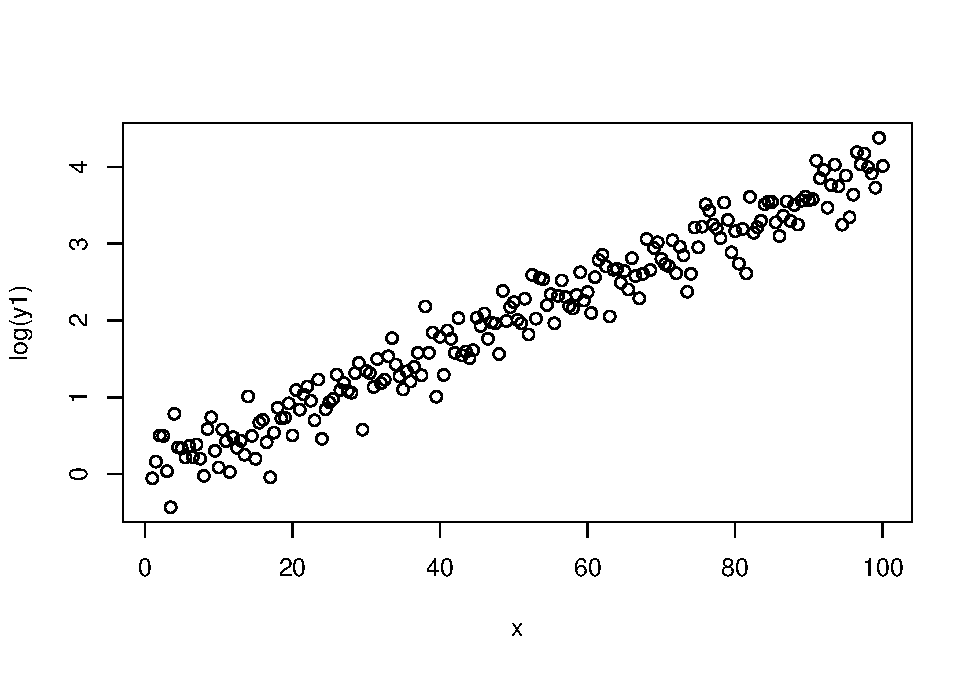
\includegraphics{Impacto_sigma_files/figure-latex/unnamed-chunk-7-1.pdf}

\begin{Shaded}
\begin{Highlighting}[]
\KeywordTok{histogram}\NormalTok{(y1)}
\KeywordTok{plotDist}\NormalTok{(}\StringTok{"lnorm"}\NormalTok{, }
         \DataTypeTok{meanlog =} \KeywordTok{mean}\NormalTok{(}\KeywordTok{log}\NormalTok{(y1), }\DataTypeTok{na.rm =} \OtherTok{TRUE}\NormalTok{),}
         \DataTypeTok{sdlog =} \KeywordTok{sd}\NormalTok{(}\KeywordTok{log}\NormalTok{(y1), }\DataTypeTok{na.rm =} \OtherTok{TRUE}\NormalTok{), }
         \DataTypeTok{add =} \OtherTok{TRUE}\NormalTok{)}
\end{Highlighting}
\end{Shaded}

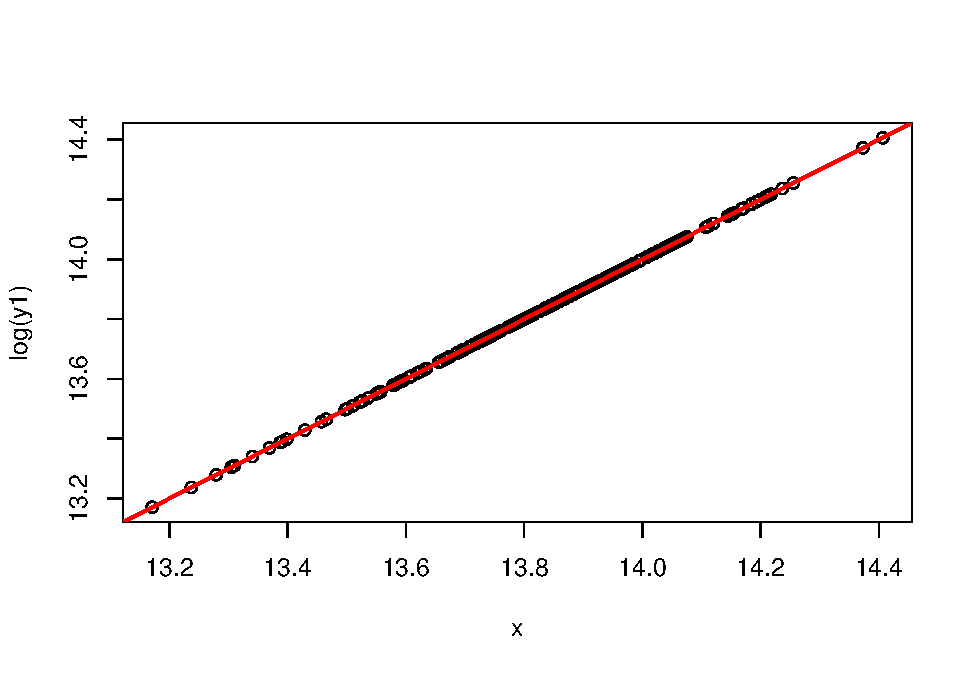
\includegraphics{Impacto_sigma_files/figure-latex/unnamed-chunk-8-1.pdf}

\subsection{MODELO}\label{modelo-1}

\begin{Shaded}
\begin{Highlighting}[]
\NormalTok{fit1 <-}\StringTok{ }\KeywordTok{lm}\NormalTok{(}\KeywordTok{log}\NormalTok{(y1) }\OperatorTok{~}\StringTok{ }\NormalTok{x)}
\NormalTok{s1 <-}\StringTok{ }\KeywordTok{summary}\NormalTok{(fit1)}
\NormalTok{s1}
\end{Highlighting}
\end{Shaded}

\begin{verbatim}
## 
## Call:
## lm(formula = log(y1) ~ x)
## 
## Residuals:
##      Min       1Q   Median       3Q      Max 
## -0.73214 -0.12672 -0.00943  0.17041  0.65261 
## 
## Coefficients:
##              Estimate Std. Error t value Pr(>|t|)    
## (Intercept) 0.0100938  0.0363167   0.278    0.781    
## x           0.0399891  0.0006251  63.972   <2e-16 ***
## ---
## Signif. codes:  0 '***' 0.001 '**' 0.01 '*' 0.05 '.' 0.1 ' ' 1
## 
## Residual standard error: 0.2533 on 197 degrees of freedom
## Multiple R-squared:  0.9541, Adjusted R-squared:  0.9538 
## F-statistic:  4092 on 1 and 197 DF,  p-value: < 2.2e-16
\end{verbatim}

\section{EXEMPLO 3}\label{exemplo-3}

Mantido mesmo vetor x criado anteriormente.

\subsection{GERAÇÃO DE DADOS
RANDÔMICOS}\label{geracao-de-dados-randomicos-2}

\begin{Shaded}
\begin{Highlighting}[]
\NormalTok{y2 <-}\StringTok{ }\KeywordTok{exp}\NormalTok{(x}\OperatorTok{/}\DecValTok{25} \OperatorTok{+}\StringTok{ }\KeywordTok{rnorm}\NormalTok{(}\DecValTok{199}\NormalTok{, }\DataTypeTok{sd =}\NormalTok{ .}\DecValTok{5}\NormalTok{)) }
\end{Highlighting}
\end{Shaded}

\subsection{GRÁFICOS}\label{graficos-2}

\begin{Shaded}
\begin{Highlighting}[]
\KeywordTok{plot}\NormalTok{(}\KeywordTok{log}\NormalTok{(y2) }\OperatorTok{~}\StringTok{ }\NormalTok{x)}
\end{Highlighting}
\end{Shaded}

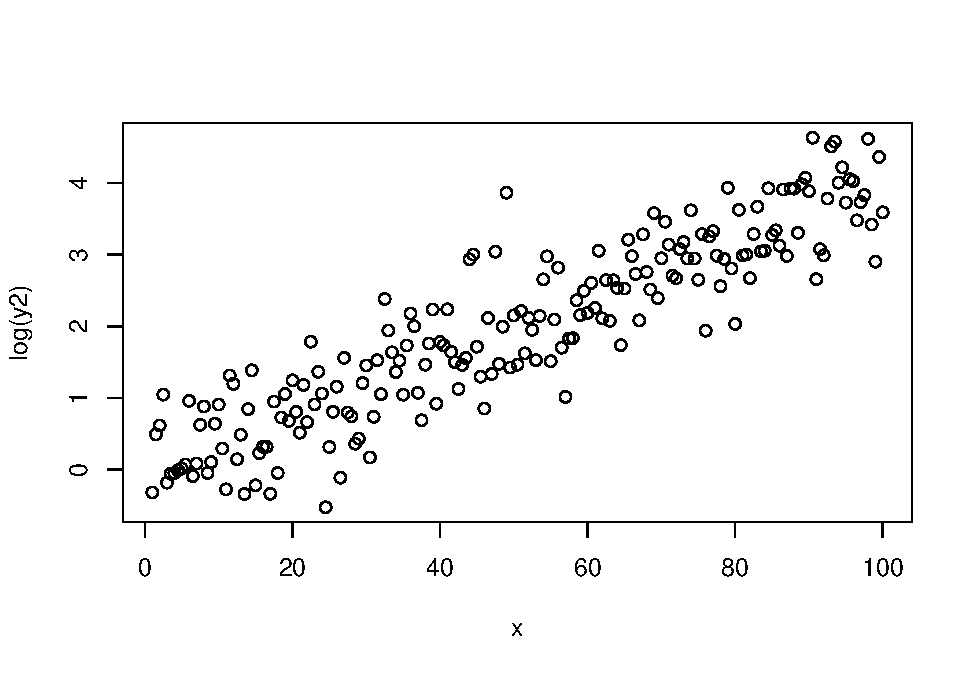
\includegraphics{Impacto_sigma_files/figure-latex/unnamed-chunk-11-1.pdf}

\begin{Shaded}
\begin{Highlighting}[]
\KeywordTok{histogram}\NormalTok{(y2)}
\KeywordTok{plotDist}\NormalTok{(}\StringTok{"lnorm"}\NormalTok{, }
         \DataTypeTok{meanlog =} \KeywordTok{mean}\NormalTok{(}\KeywordTok{log}\NormalTok{(y2), }\DataTypeTok{na.rm =} \OtherTok{TRUE}\NormalTok{),}
         \DataTypeTok{sdlog =} \KeywordTok{sd}\NormalTok{(}\KeywordTok{log}\NormalTok{(y2), }\DataTypeTok{na.rm =} \OtherTok{TRUE}\NormalTok{), }
         \DataTypeTok{add =} \OtherTok{TRUE}\NormalTok{)}
\end{Highlighting}
\end{Shaded}

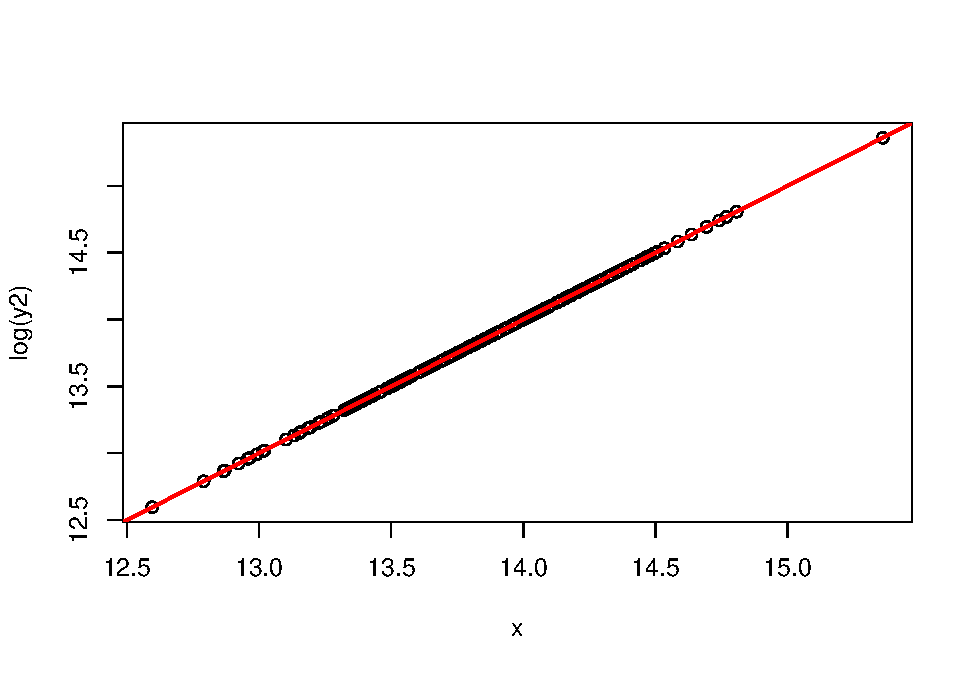
\includegraphics{Impacto_sigma_files/figure-latex/unnamed-chunk-12-1.pdf}

\subsection{MODELO}\label{modelo-2}

\begin{Shaded}
\begin{Highlighting}[]
\NormalTok{fit2 <-}\StringTok{ }\KeywordTok{lm}\NormalTok{(}\KeywordTok{log}\NormalTok{(y2) }\OperatorTok{~}\StringTok{ }\NormalTok{x)}
\NormalTok{s2 <-}\StringTok{ }\KeywordTok{summary}\NormalTok{(fit2)}
\NormalTok{s2}
\end{Highlighting}
\end{Shaded}

\begin{verbatim}
## 
## Call:
## lm(formula = log(y2) ~ x)
## 
## Residuals:
##     Min      1Q  Median      3Q     Max 
## -1.4740 -0.3438 -0.0224  0.3471  1.9256 
## 
## Coefficients:
##              Estimate Std. Error t value Pr(>|t|)    
## (Intercept) -0.039644   0.077034  -0.515    0.607    
## x            0.040391   0.001326  30.462   <2e-16 ***
## ---
## Signif. codes:  0 '***' 0.001 '**' 0.01 '*' 0.05 '.' 0.1 ' ' 1
## 
## Residual standard error: 0.5373 on 197 degrees of freedom
## Multiple R-squared:  0.8249, Adjusted R-squared:  0.824 
## F-statistic: 927.9 on 1 and 197 DF,  p-value: < 2.2e-16
\end{verbatim}

\section{EXEMPLO 4}\label{exemplo-4}

Mantido mesmo vetor x criado anteriormente.

\subsection{GERAÇÃO DE DADOS
RANDÔMICOS}\label{geracao-de-dados-randomicos-3}

\begin{Shaded}
\begin{Highlighting}[]
\NormalTok{y3 <-}\StringTok{ }\KeywordTok{exp}\NormalTok{(x}\OperatorTok{/}\DecValTok{25} \OperatorTok{+}\StringTok{ }\KeywordTok{rnorm}\NormalTok{(}\DecValTok{199}\NormalTok{, }\DataTypeTok{sd =}\NormalTok{ .}\DecValTok{75}\NormalTok{)) }
\end{Highlighting}
\end{Shaded}

\subsection{GRÁFICOS}\label{graficos-3}

\begin{Shaded}
\begin{Highlighting}[]
\KeywordTok{plot}\NormalTok{(}\KeywordTok{log}\NormalTok{(y3) }\OperatorTok{~}\StringTok{ }\NormalTok{x)}
\end{Highlighting}
\end{Shaded}

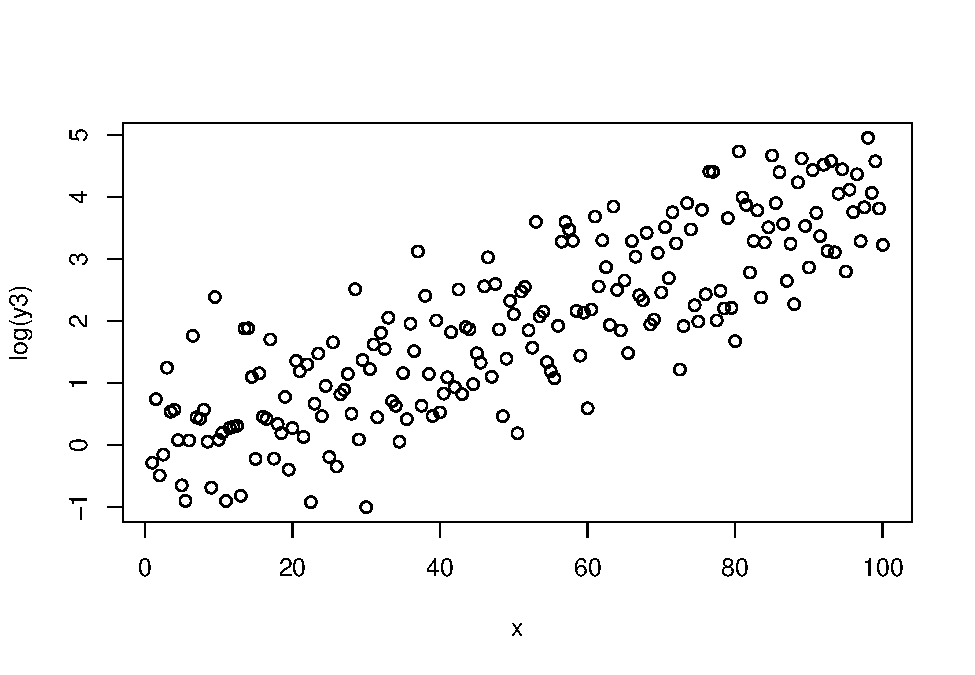
\includegraphics{Impacto_sigma_files/figure-latex/unnamed-chunk-15-1.pdf}

\begin{Shaded}
\begin{Highlighting}[]
\KeywordTok{histogram}\NormalTok{(y3)}
\KeywordTok{plotDist}\NormalTok{(}\StringTok{"lnorm"}\NormalTok{, }
         \DataTypeTok{meanlog =} \KeywordTok{mean}\NormalTok{(}\KeywordTok{log}\NormalTok{(y3), }\DataTypeTok{na.rm =} \OtherTok{TRUE}\NormalTok{),}
         \DataTypeTok{sdlog =} \KeywordTok{sd}\NormalTok{(}\KeywordTok{log}\NormalTok{(y3), }\DataTypeTok{na.rm =} \OtherTok{TRUE}\NormalTok{), }
         \DataTypeTok{add =} \OtherTok{TRUE}\NormalTok{)}
\end{Highlighting}
\end{Shaded}

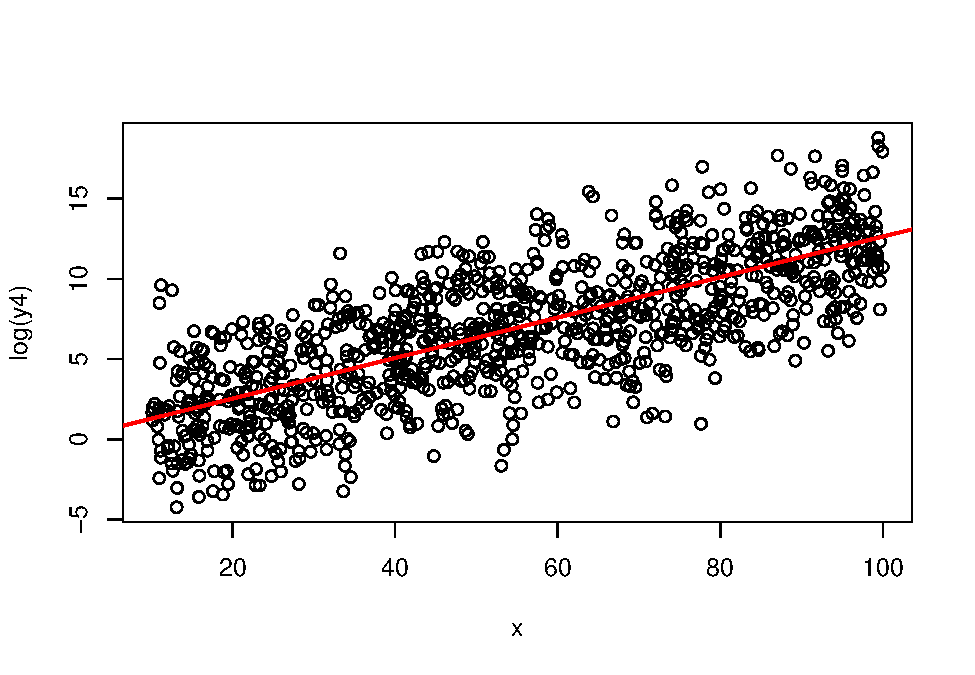
\includegraphics{Impacto_sigma_files/figure-latex/unnamed-chunk-16-1.pdf}

\subsection{MODELO}\label{modelo-3}

\begin{Shaded}
\begin{Highlighting}[]
\NormalTok{fit3 <-}\StringTok{ }\KeywordTok{lm}\NormalTok{(}\KeywordTok{log}\NormalTok{(y3) }\OperatorTok{~}\StringTok{ }\NormalTok{x)}
\NormalTok{s3 <-}\StringTok{ }\KeywordTok{summary}\NormalTok{(fit3)}
\NormalTok{s3}
\end{Highlighting}
\end{Shaded}

\begin{verbatim}
## 
## Call:
## lm(formula = log(y3) ~ x)
## 
## Residuals:
##      Min       1Q   Median       3Q      Max 
## -2.09563 -0.64150 -0.03851  0.59729  2.15902 
## 
## Coefficients:
##              Estimate Std. Error t value Pr(>|t|)    
## (Intercept) -0.172145   0.115687  -1.488    0.138    
## x            0.042098   0.001991  21.141   <2e-16 ***
## ---
## Signif. codes:  0 '***' 0.001 '**' 0.01 '*' 0.05 '.' 0.1 ' ' 1
## 
## Residual standard error: 0.8068 on 197 degrees of freedom
## Multiple R-squared:  0.6941, Adjusted R-squared:  0.6925 
## F-statistic:   447 on 1 and 197 DF,  p-value: < 2.2e-16
\end{verbatim}

\section{EXEMPLO 5}\label{exemplo-5}

Mantido mesmo vetor x criado anteriormente.

\subsection{GERAÇÃO DE DADOS
RANDÔMICOS}\label{geracao-de-dados-randomicos-4}

\begin{Shaded}
\begin{Highlighting}[]
\NormalTok{y4 <-}\StringTok{ }\KeywordTok{exp}\NormalTok{(x}\OperatorTok{/}\DecValTok{25} \OperatorTok{+}\StringTok{ }\KeywordTok{rnorm}\NormalTok{(}\DecValTok{199}\NormalTok{, }\DataTypeTok{sd =} \DecValTok{1}\NormalTok{)) }
\end{Highlighting}
\end{Shaded}

\subsection{GRÁFICOS}\label{graficos-4}

\begin{Shaded}
\begin{Highlighting}[]
\KeywordTok{plot}\NormalTok{(}\KeywordTok{log}\NormalTok{(y4) }\OperatorTok{~}\StringTok{ }\NormalTok{x)}
\end{Highlighting}
\end{Shaded}

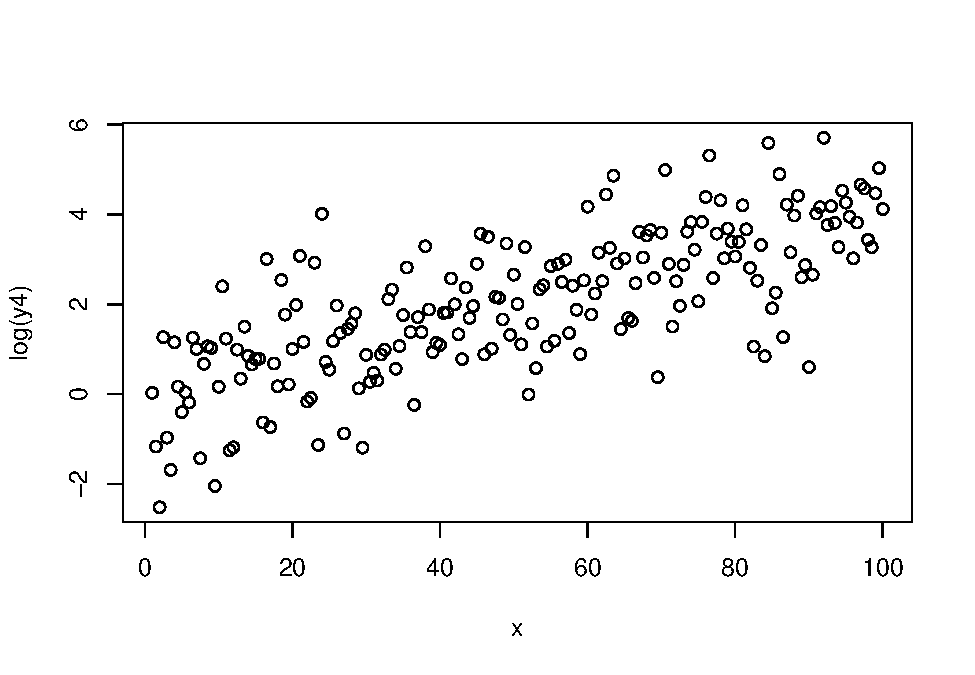
\includegraphics{Impacto_sigma_files/figure-latex/unnamed-chunk-19-1.pdf}

\begin{Shaded}
\begin{Highlighting}[]
\KeywordTok{histogram}\NormalTok{(y4)}
\KeywordTok{plotDist}\NormalTok{(}\StringTok{"lnorm"}\NormalTok{, }
         \DataTypeTok{meanlog =} \KeywordTok{mean}\NormalTok{(}\KeywordTok{log}\NormalTok{(y4), }\DataTypeTok{na.rm =} \OtherTok{TRUE}\NormalTok{),}
         \DataTypeTok{sdlog =} \KeywordTok{sd}\NormalTok{(}\KeywordTok{log}\NormalTok{(y4), }\DataTypeTok{na.rm =} \OtherTok{TRUE}\NormalTok{), }
         \DataTypeTok{add =} \OtherTok{TRUE}\NormalTok{)}
\end{Highlighting}
\end{Shaded}

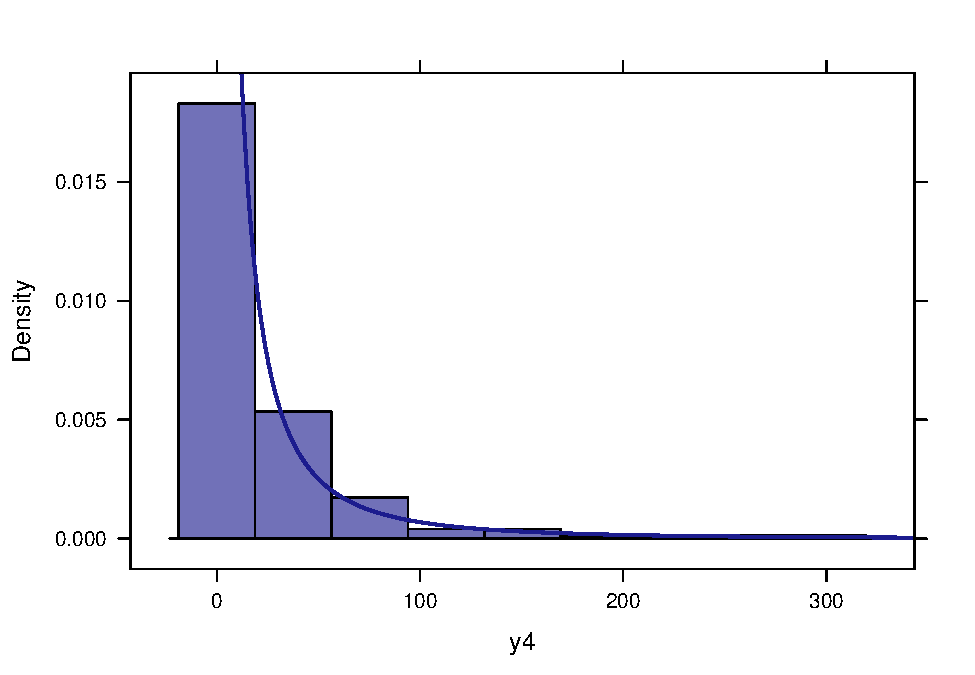
\includegraphics{Impacto_sigma_files/figure-latex/unnamed-chunk-20-1.pdf}

\subsection{MODELO}\label{modelo-4}

\begin{Shaded}
\begin{Highlighting}[]
\NormalTok{fit4 <-}\StringTok{ }\KeywordTok{lm}\NormalTok{(}\KeywordTok{log}\NormalTok{(y4) }\OperatorTok{~}\StringTok{ }\NormalTok{x)}
\NormalTok{s4 <-}\StringTok{ }\KeywordTok{summary}\NormalTok{(fit4)}
\NormalTok{s4}
\end{Highlighting}
\end{Shaded}

\begin{verbatim}
## 
## Call:
## lm(formula = log(y4) ~ x)
## 
## Residuals:
##      Min       1Q   Median       3Q      Max 
## -3.07159 -0.71233  0.07082  0.67517  3.08445 
## 
## Coefficients:
##              Estimate Std. Error t value Pr(>|t|)    
## (Intercept) -0.066296   0.155891  -0.425    0.671    
## x            0.041566   0.002683  15.491   <2e-16 ***
## ---
## Signif. codes:  0 '***' 0.001 '**' 0.01 '*' 0.05 '.' 0.1 ' ' 1
## 
## Residual standard error: 1.087 on 197 degrees of freedom
## Multiple R-squared:  0.5492, Adjusted R-squared:  0.5469 
## F-statistic:   240 on 1 and 197 DF,  p-value: < 2.2e-16
\end{verbatim}

\section{ESTIMATIVAS}\label{estimativas}

\subsection{Usando o primeiro modelo}\label{usando-o-primeiro-modelo}

\begin{enumerate}
\def\labelenumi{\alph{enumi}.}
\tightlist
\item
  Moda
\end{enumerate}

\begin{Shaded}
\begin{Highlighting}[]
\NormalTok{p <-}\StringTok{ }\KeywordTok{predict}\NormalTok{(fit, }\DataTypeTok{newdata =} \KeywordTok{data.frame}\NormalTok{(}\DataTypeTok{x =} \DecValTok{50}\NormalTok{))}
\NormalTok{p_moda <-}\StringTok{ }\KeywordTok{exp}\NormalTok{(p }\OperatorTok{-}\StringTok{ }\NormalTok{s}\OperatorTok{$}\NormalTok{sigma}\OperatorTok{^}\DecValTok{2}\NormalTok{)}
\NormalTok{p_moda}
\end{Highlighting}
\end{Shaded}

\begin{verbatim}
##        1 
## 7.353577
\end{verbatim}

\begin{enumerate}
\def\labelenumi{\alph{enumi}.}
\setcounter{enumi}{1}
\tightlist
\item
  Mediana
\end{enumerate}

\begin{Shaded}
\begin{Highlighting}[]
\NormalTok{p_mediana <-}\StringTok{ }\KeywordTok{exp}\NormalTok{(p)}
\NormalTok{p_mediana}
\end{Highlighting}
\end{Shaded}

\begin{verbatim}
##        1 
## 7.417663
\end{verbatim}

\begin{enumerate}
\def\labelenumi{\alph{enumi}.}
\setcounter{enumi}{2}
\tightlist
\item
  Média
\end{enumerate}

\begin{Shaded}
\begin{Highlighting}[]
\NormalTok{p_media <-}\StringTok{ }\KeywordTok{exp}\NormalTok{(p }\OperatorTok{+}\StringTok{ }\NormalTok{s}\OperatorTok{$}\NormalTok{sigma}\OperatorTok{^}\DecValTok{2}\OperatorTok{/}\DecValTok{2}\NormalTok{)}
\NormalTok{p_media}
\end{Highlighting}
\end{Shaded}

\begin{verbatim}
##        1 
## 7.449915
\end{verbatim}

\subsection{Usando o segundo modelo}\label{usando-o-segundo-modelo}

\begin{enumerate}
\def\labelenumi{\alph{enumi}.}
\tightlist
\item
  Moda
\end{enumerate}

\begin{Shaded}
\begin{Highlighting}[]
\NormalTok{p1 <-}\StringTok{ }\KeywordTok{predict}\NormalTok{(fit1, }\DataTypeTok{newdata =} \KeywordTok{data.frame}\NormalTok{(}\DataTypeTok{x =} \DecValTok{50}\NormalTok{))}
\NormalTok{p1_moda <-}\StringTok{ }\KeywordTok{exp}\NormalTok{(p1 }\OperatorTok{-}\StringTok{ }\NormalTok{s1}\OperatorTok{$}\NormalTok{sigma}\OperatorTok{^}\DecValTok{2}\NormalTok{)}
\NormalTok{p1_moda}
\end{Highlighting}
\end{Shaded}

\begin{verbatim}
##        1 
## 6.996403
\end{verbatim}

\begin{enumerate}
\def\labelenumi{\alph{enumi}.}
\setcounter{enumi}{1}
\tightlist
\item
  Mediana
\end{enumerate}

\begin{Shaded}
\begin{Highlighting}[]
\NormalTok{p1_mediana <-}\StringTok{ }\KeywordTok{exp}\NormalTok{(p1)}
\NormalTok{p1_mediana}
\end{Highlighting}
\end{Shaded}

\begin{verbatim}
##        1 
## 7.459949
\end{verbatim}

\begin{enumerate}
\def\labelenumi{\alph{enumi}.}
\setcounter{enumi}{2}
\tightlist
\item
  Média
\end{enumerate}

\begin{Shaded}
\begin{Highlighting}[]
\NormalTok{p1_media <-}\StringTok{ }\KeywordTok{exp}\NormalTok{(p1 }\OperatorTok{+}\StringTok{ }\NormalTok{s1}\OperatorTok{$}\NormalTok{sigma}\OperatorTok{^}\DecValTok{2}\OperatorTok{/}\DecValTok{2}\NormalTok{)}
\NormalTok{p1_media}
\end{Highlighting}
\end{Shaded}

\begin{verbatim}
##        1 
## 7.703116
\end{verbatim}

\subsection{Usando o terceiro modelo}\label{usando-o-terceiro-modelo}

\begin{enumerate}
\def\labelenumi{\alph{enumi}.}
\tightlist
\item
  Moda
\end{enumerate}

\begin{Shaded}
\begin{Highlighting}[]
\NormalTok{p2 <-}\StringTok{ }\KeywordTok{predict}\NormalTok{(fit2, }\DataTypeTok{newdata =} \KeywordTok{data.frame}\NormalTok{(}\DataTypeTok{x =} \DecValTok{50}\NormalTok{))}
\NormalTok{p2_moda <-}\StringTok{ }\KeywordTok{exp}\NormalTok{(p2 }\OperatorTok{-}\StringTok{ }\NormalTok{s2}\OperatorTok{$}\NormalTok{sigma}\OperatorTok{^}\DecValTok{2}\NormalTok{)}
\NormalTok{p2_moda}
\end{Highlighting}
\end{Shaded}

\begin{verbatim}
##        1 
## 5.426298
\end{verbatim}

\begin{enumerate}
\def\labelenumi{\alph{enumi}.}
\setcounter{enumi}{1}
\tightlist
\item
  Mediana
\end{enumerate}

\begin{Shaded}
\begin{Highlighting}[]
\NormalTok{p2_mediana <-}\StringTok{ }\KeywordTok{exp}\NormalTok{(p2)}
\NormalTok{p2_mediana}
\end{Highlighting}
\end{Shaded}

\begin{verbatim}
##        1 
## 7.242041
\end{verbatim}

\begin{enumerate}
\def\labelenumi{\alph{enumi}.}
\setcounter{enumi}{2}
\tightlist
\item
  Média
\end{enumerate}

\begin{Shaded}
\begin{Highlighting}[]
\NormalTok{p2_media <-}\StringTok{ }\KeywordTok{exp}\NormalTok{(p2 }\OperatorTok{+}\StringTok{ }\NormalTok{s2}\OperatorTok{$}\NormalTok{sigma}\OperatorTok{^}\DecValTok{2}\OperatorTok{/}\DecValTok{2}\NormalTok{)}
\NormalTok{p2_media}
\end{Highlighting}
\end{Shaded}

\begin{verbatim}
##       1 
## 8.36642
\end{verbatim}

\subsection{Usando o quarto modelo}\label{usando-o-quarto-modelo}

\begin{enumerate}
\def\labelenumi{\alph{enumi}.}
\tightlist
\item
  Moda
\end{enumerate}

\begin{Shaded}
\begin{Highlighting}[]
\NormalTok{p3 <-}\StringTok{ }\KeywordTok{predict}\NormalTok{(fit3, }\DataTypeTok{newdata =} \KeywordTok{data.frame}\NormalTok{(}\DataTypeTok{x =} \DecValTok{50}\NormalTok{))}
\NormalTok{p3_moda <-}\StringTok{ }\KeywordTok{exp}\NormalTok{(p3 }\OperatorTok{-}\StringTok{ }\NormalTok{s3}\OperatorTok{$}\NormalTok{sigma}\OperatorTok{^}\DecValTok{2}\NormalTok{)}
\NormalTok{p3_moda}
\end{Highlighting}
\end{Shaded}

\begin{verbatim}
##        1 
## 3.603033
\end{verbatim}

\begin{enumerate}
\def\labelenumi{\alph{enumi}.}
\setcounter{enumi}{1}
\tightlist
\item
  Mediana
\end{enumerate}

\begin{Shaded}
\begin{Highlighting}[]
\NormalTok{p3_mediana <-}\StringTok{ }\KeywordTok{exp}\NormalTok{(p3)}
\NormalTok{p3_mediana}
\end{Highlighting}
\end{Shaded}

\begin{verbatim}
##        1 
## 6.908516
\end{verbatim}

\begin{enumerate}
\def\labelenumi{\alph{enumi}.}
\setcounter{enumi}{2}
\tightlist
\item
  Média
\end{enumerate}

\begin{Shaded}
\begin{Highlighting}[]
\NormalTok{p3_media <-}\StringTok{ }\KeywordTok{exp}\NormalTok{(p3 }\OperatorTok{+}\StringTok{ }\NormalTok{s3}\OperatorTok{$}\NormalTok{sigma}\OperatorTok{^}\DecValTok{2}\OperatorTok{/}\DecValTok{2}\NormalTok{)}
\NormalTok{p3_media}
\end{Highlighting}
\end{Shaded}

\begin{verbatim}
##        1 
## 9.566278
\end{verbatim}

\subsection{Usando o quinto modelo}\label{usando-o-quinto-modelo}

\begin{enumerate}
\def\labelenumi{\alph{enumi}.}
\tightlist
\item
  Moda
\end{enumerate}

\begin{Shaded}
\begin{Highlighting}[]
\NormalTok{p4 <-}\StringTok{ }\KeywordTok{predict}\NormalTok{(fit4, }\DataTypeTok{newdata =} \KeywordTok{data.frame}\NormalTok{(}\DataTypeTok{x =} \DecValTok{50}\NormalTok{))}
\NormalTok{p4_moda <-}\StringTok{ }\KeywordTok{exp}\NormalTok{(p4 }\OperatorTok{-}\StringTok{ }\NormalTok{s4}\OperatorTok{$}\NormalTok{sigma}\OperatorTok{^}\DecValTok{2}\NormalTok{)}
\NormalTok{p4_moda}
\end{Highlighting}
\end{Shaded}

\begin{verbatim}
##        1 
## 2.293168
\end{verbatim}

\begin{enumerate}
\def\labelenumi{\alph{enumi}.}
\setcounter{enumi}{1}
\tightlist
\item
  Mediana
\end{enumerate}

\begin{Shaded}
\begin{Highlighting}[]
\NormalTok{p4_mediana <-}\StringTok{ }\KeywordTok{exp}\NormalTok{(p4)}
\NormalTok{p4_mediana}
\end{Highlighting}
\end{Shaded}

\begin{verbatim}
##       1 
## 7.47829
\end{verbatim}

\begin{enumerate}
\def\labelenumi{\alph{enumi}.}
\setcounter{enumi}{2}
\tightlist
\item
  Média
\end{enumerate}

\begin{Shaded}
\begin{Highlighting}[]
\NormalTok{p4_media <-}\StringTok{ }\KeywordTok{exp}\NormalTok{(p4 }\OperatorTok{+}\StringTok{ }\NormalTok{s4}\OperatorTok{$}\NormalTok{sigma}\OperatorTok{^}\DecValTok{2}\OperatorTok{/}\DecValTok{2}\NormalTok{)}
\NormalTok{p4_media}
\end{Highlighting}
\end{Shaded}

\begin{verbatim}
##        1 
## 13.50472
\end{verbatim}

\section{VISUALIZAÇÃO GRÁFICA}\label{visualizacao-grafica}

\begin{Shaded}
\begin{Highlighting}[]
\NormalTok{df <-}\StringTok{ }\KeywordTok{data.frame}\NormalTok{(}\DataTypeTok{sd =} \KeywordTok{c}\NormalTok{(}\FloatTok{0.1}\NormalTok{, }\FloatTok{0.25}\NormalTok{, }\FloatTok{0.5}\NormalTok{, }\FloatTok{0.75}\NormalTok{, }\DecValTok{1}\NormalTok{),}
                 \DataTypeTok{moda =} \KeywordTok{c}\NormalTok{(p_moda, p1_moda, p2_moda, p3_moda, p4_moda),}
                 \DataTypeTok{mediana =} \KeywordTok{c}\NormalTok{(p_mediana, p1_mediana, p2_mediana, p3_mediana, p4_mediana),}
                 \DataTypeTok{media =} \KeywordTok{c}\NormalTok{(p_media, p1_media, p2_media, p3_media, p4_media))}
\NormalTok{df <-}\StringTok{ }\KeywordTok{melt}\NormalTok{(df, }\DataTypeTok{id =} \StringTok{"sd"}\NormalTok{)}
\end{Highlighting}
\end{Shaded}

\begin{Shaded}
\begin{Highlighting}[]
\KeywordTok{ggplot}\NormalTok{(df, }\KeywordTok{aes}\NormalTok{(}\DataTypeTok{x =}\NormalTok{ sd, }\DataTypeTok{y =}\NormalTok{ value, }\DataTypeTok{color =}\NormalTok{ variable)) }\OperatorTok{+}\StringTok{ }
\StringTok{  }\KeywordTok{geom_point}\NormalTok{() }\OperatorTok{+}\StringTok{ }\KeywordTok{geom_line}\NormalTok{()}
\end{Highlighting}
\end{Shaded}

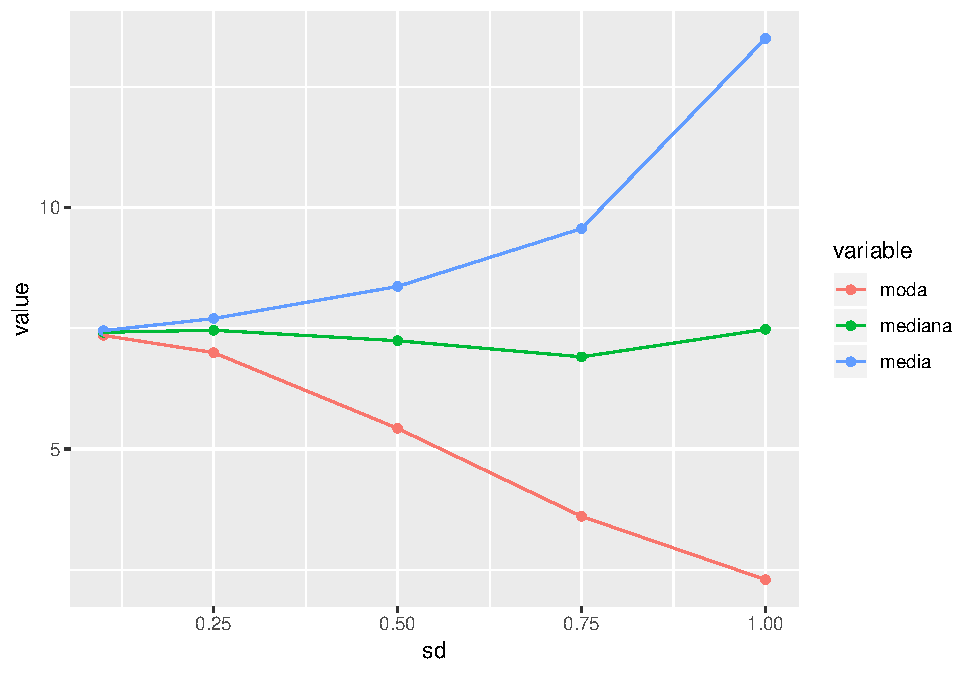
\includegraphics{Impacto_sigma_files/figure-latex/unnamed-chunk-38-1.pdf}

\section{VALIDAÇÃO CRUZADA}\label{validacao-cruzada}

\subsection{Modelo 1}\label{modelo-1-1}

\begin{Shaded}
\begin{Highlighting}[]
\NormalTok{id <-}\StringTok{ }\KeywordTok{sample}\NormalTok{(}\DecValTok{1}\OperatorTok{:}\DecValTok{199}\NormalTok{, }\DecValTok{139}\NormalTok{)}
\NormalTok{y_train <-}\StringTok{ }\NormalTok{y[id]}
\NormalTok{y_test <-}\StringTok{  }\NormalTok{y[}\OperatorTok{-}\NormalTok{id]}
\NormalTok{x_train <-}\StringTok{ }\NormalTok{x[id]}
\NormalTok{fit <-}\StringTok{ }\KeywordTok{lm}\NormalTok{(}\KeywordTok{log}\NormalTok{(y_train) }\OperatorTok{~}\StringTok{ }\NormalTok{x_train)}
\NormalTok{s <-}\StringTok{ }\KeywordTok{summary}\NormalTok{(fit)}
\NormalTok{p <-}\StringTok{ }\KeywordTok{predict}\NormalTok{(fit, }\DataTypeTok{newdata =} \KeywordTok{data.frame}\NormalTok{(}\DataTypeTok{x_train =}\NormalTok{ x[}\OperatorTok{-}\NormalTok{id]))}
\NormalTok{p_moda <-}\StringTok{ }\KeywordTok{exp}\NormalTok{(p }\OperatorTok{-}\StringTok{ }\NormalTok{s}\OperatorTok{$}\NormalTok{sigma}\OperatorTok{^}\DecValTok{2}\NormalTok{)}
\NormalTok{p_mediana <-}\StringTok{ }\KeywordTok{exp}\NormalTok{(p)}
\NormalTok{p_media <-}\StringTok{ }\KeywordTok{exp}\NormalTok{(p }\OperatorTok{+}\StringTok{ }\NormalTok{s}\OperatorTok{$}\NormalTok{sigma}\OperatorTok{^}\DecValTok{2}\OperatorTok{/}\DecValTok{2}\NormalTok{)}
\NormalTok{(rmse_moda <-}\StringTok{ }\KeywordTok{sqrt}\NormalTok{(}\KeywordTok{mean}\NormalTok{((p_moda }\OperatorTok{-}\StringTok{ }\NormalTok{y_test)}\OperatorTok{^}\DecValTok{2}\NormalTok{)))}
\end{Highlighting}
\end{Shaded}

\begin{verbatim}
## [1] 1.957474
\end{verbatim}

\begin{Shaded}
\begin{Highlighting}[]
\NormalTok{(rmse_mediana <-}\StringTok{ }\KeywordTok{sqrt}\NormalTok{(}\KeywordTok{mean}\NormalTok{((p_mediana }\OperatorTok{-}\StringTok{ }\NormalTok{y_test)}\OperatorTok{^}\DecValTok{2}\NormalTok{)))}
\end{Highlighting}
\end{Shaded}

\begin{verbatim}
## [1] 1.891117
\end{verbatim}

\begin{Shaded}
\begin{Highlighting}[]
\NormalTok{(rmse_media <-}\StringTok{ }\KeywordTok{sqrt}\NormalTok{(}\KeywordTok{mean}\NormalTok{((p_media }\OperatorTok{-}\StringTok{ }\NormalTok{y_test)}\OperatorTok{^}\DecValTok{2}\NormalTok{)))}
\end{Highlighting}
\end{Shaded}

\begin{verbatim}
## [1] 1.863776
\end{verbatim}

\subsection{Modelo 2}\label{modelo-2-1}

\begin{Shaded}
\begin{Highlighting}[]
\NormalTok{id <-}\StringTok{ }\KeywordTok{sample}\NormalTok{(}\DecValTok{1}\OperatorTok{:}\DecValTok{199}\NormalTok{, }\DecValTok{139}\NormalTok{)}
\NormalTok{y1_train <-}\StringTok{ }\NormalTok{y1[id]}
\NormalTok{y1_test <-}\StringTok{  }\NormalTok{y1[}\OperatorTok{-}\NormalTok{id]}
\NormalTok{x_train <-}\StringTok{ }\NormalTok{x[id]}
\NormalTok{fit1 <-}\StringTok{ }\KeywordTok{lm}\NormalTok{(}\KeywordTok{log}\NormalTok{(y1_train) }\OperatorTok{~}\StringTok{ }\NormalTok{x_train)}
\NormalTok{s1 <-}\StringTok{ }\KeywordTok{summary}\NormalTok{(fit1)}
\NormalTok{p1 <-}\StringTok{ }\KeywordTok{predict}\NormalTok{(fit1, }\DataTypeTok{newdata =} \KeywordTok{data.frame}\NormalTok{(}\DataTypeTok{x_train =}\NormalTok{ x[}\OperatorTok{-}\NormalTok{id]))}
\NormalTok{p1_moda <-}\StringTok{ }\KeywordTok{exp}\NormalTok{(p1 }\OperatorTok{-}\StringTok{ }\NormalTok{s1}\OperatorTok{$}\NormalTok{sigma}\OperatorTok{^}\DecValTok{2}\NormalTok{)}
\NormalTok{p1_mediana <-}\StringTok{ }\KeywordTok{exp}\NormalTok{(p1)}
\NormalTok{p1_media <-}\StringTok{ }\KeywordTok{exp}\NormalTok{(p1 }\OperatorTok{+}\StringTok{ }\NormalTok{s1}\OperatorTok{$}\NormalTok{sigma}\OperatorTok{^}\DecValTok{2}\OperatorTok{/}\DecValTok{2}\NormalTok{)}
\NormalTok{(rmse1_moda <-}\StringTok{ }\KeywordTok{sqrt}\NormalTok{(}\KeywordTok{mean}\NormalTok{((p1_moda }\OperatorTok{-}\StringTok{ }\NormalTok{y1_test)}\OperatorTok{^}\DecValTok{2}\NormalTok{)))}
\end{Highlighting}
\end{Shaded}

\begin{verbatim}
## [1] 5.480126
\end{verbatim}

\begin{Shaded}
\begin{Highlighting}[]
\NormalTok{(rmse1_mediana <-}\StringTok{ }\KeywordTok{sqrt}\NormalTok{(}\KeywordTok{mean}\NormalTok{((p1_mediana }\OperatorTok{-}\StringTok{ }\NormalTok{y1_test)}\OperatorTok{^}\DecValTok{2}\NormalTok{)))}
\end{Highlighting}
\end{Shaded}

\begin{verbatim}
## [1] 5.111089
\end{verbatim}

\begin{Shaded}
\begin{Highlighting}[]
\NormalTok{(rmse1_media <-}\StringTok{ }\KeywordTok{sqrt}\NormalTok{(}\KeywordTok{mean}\NormalTok{((p1_media }\OperatorTok{-}\StringTok{ }\NormalTok{y1_test)}\OperatorTok{^}\DecValTok{2}\NormalTok{)))}
\end{Highlighting}
\end{Shaded}

\begin{verbatim}
## [1] 5.080717
\end{verbatim}

\subsection{Modelo 3}\label{modelo-3-1}

\begin{Shaded}
\begin{Highlighting}[]
\NormalTok{id <-}\StringTok{ }\KeywordTok{sample}\NormalTok{(}\DecValTok{1}\OperatorTok{:}\DecValTok{199}\NormalTok{, }\DecValTok{139}\NormalTok{)}
\NormalTok{y2_train <-}\StringTok{ }\NormalTok{y2[id]}
\NormalTok{y2_test <-}\StringTok{  }\NormalTok{y2[}\OperatorTok{-}\NormalTok{id]}
\NormalTok{x_train <-}\StringTok{ }\NormalTok{x[id]}
\NormalTok{fit2 <-}\StringTok{ }\KeywordTok{lm}\NormalTok{(}\KeywordTok{log}\NormalTok{(y2_train) }\OperatorTok{~}\StringTok{ }\NormalTok{x_train)}
\NormalTok{s2 <-}\StringTok{ }\KeywordTok{summary}\NormalTok{(fit2)}
\NormalTok{p2 <-}\StringTok{ }\KeywordTok{predict}\NormalTok{(fit2, }\DataTypeTok{newdata =} \KeywordTok{data.frame}\NormalTok{(}\DataTypeTok{x_train =}\NormalTok{ x[}\OperatorTok{-}\NormalTok{id]))}
\NormalTok{p2_moda <-}\StringTok{ }\KeywordTok{exp}\NormalTok{(p2 }\OperatorTok{-}\StringTok{ }\NormalTok{s2}\OperatorTok{$}\NormalTok{sigma}\OperatorTok{^}\DecValTok{2}\NormalTok{)}
\NormalTok{p2_mediana <-}\StringTok{ }\KeywordTok{exp}\NormalTok{(p2)}
\NormalTok{p2_media <-}\StringTok{ }\KeywordTok{exp}\NormalTok{(p2 }\OperatorTok{+}\StringTok{ }\NormalTok{s2}\OperatorTok{$}\NormalTok{sigma}\OperatorTok{^}\DecValTok{2}\OperatorTok{/}\DecValTok{2}\NormalTok{)}
\NormalTok{(rmse2_moda <-}\StringTok{ }\KeywordTok{sqrt}\NormalTok{(}\KeywordTok{mean}\NormalTok{((p2_moda }\OperatorTok{-}\StringTok{ }\NormalTok{y2_test)}\OperatorTok{^}\DecValTok{2}\NormalTok{)))}
\end{Highlighting}
\end{Shaded}

\begin{verbatim}
## [1] 18.19711
\end{verbatim}

\begin{Shaded}
\begin{Highlighting}[]
\NormalTok{(rmse2_mediana <-}\StringTok{ }\KeywordTok{sqrt}\NormalTok{(}\KeywordTok{mean}\NormalTok{((p2_mediana }\OperatorTok{-}\StringTok{ }\NormalTok{y2_test)}\OperatorTok{^}\DecValTok{2}\NormalTok{)))}
\end{Highlighting}
\end{Shaded}

\begin{verbatim}
## [1] 15.21072
\end{verbatim}

\begin{Shaded}
\begin{Highlighting}[]
\NormalTok{(rmse2_media <-}\StringTok{ }\KeywordTok{sqrt}\NormalTok{(}\KeywordTok{mean}\NormalTok{((p2_media }\OperatorTok{-}\StringTok{ }\NormalTok{y2_test)}\OperatorTok{^}\DecValTok{2}\NormalTok{)))}
\end{Highlighting}
\end{Shaded}

\begin{verbatim}
## [1] 13.83019
\end{verbatim}

\subsection{Modelo 4}\label{modelo-4-1}

\begin{Shaded}
\begin{Highlighting}[]
\NormalTok{id <-}\StringTok{ }\KeywordTok{sample}\NormalTok{(}\DecValTok{1}\OperatorTok{:}\DecValTok{199}\NormalTok{, }\DecValTok{139}\NormalTok{)}
\NormalTok{y3_train <-}\StringTok{ }\NormalTok{y3[id]}
\NormalTok{y3_test <-}\StringTok{  }\NormalTok{y3[}\OperatorTok{-}\NormalTok{id]}
\NormalTok{x_train <-}\StringTok{ }\NormalTok{x[id]}
\NormalTok{fit3 <-}\StringTok{ }\KeywordTok{lm}\NormalTok{(}\KeywordTok{log}\NormalTok{(y3_train) }\OperatorTok{~}\StringTok{ }\NormalTok{x_train)}
\NormalTok{s3 <-}\StringTok{ }\KeywordTok{summary}\NormalTok{(fit3)}
\NormalTok{p <-}\StringTok{ }\KeywordTok{predict}\NormalTok{(fit3, }\DataTypeTok{newdata =} \KeywordTok{data.frame}\NormalTok{(}\DataTypeTok{x_train =}\NormalTok{ x[}\OperatorTok{-}\NormalTok{id]))}
\NormalTok{p3_moda <-}\StringTok{ }\KeywordTok{exp}\NormalTok{(p3 }\OperatorTok{-}\StringTok{ }\NormalTok{s3}\OperatorTok{$}\NormalTok{sigma}\OperatorTok{^}\DecValTok{2}\NormalTok{)}
\NormalTok{p3_mediana <-}\StringTok{ }\KeywordTok{exp}\NormalTok{(p3)}
\NormalTok{p3_media <-}\StringTok{ }\KeywordTok{exp}\NormalTok{(p3 }\OperatorTok{+}\StringTok{ }\NormalTok{s3}\OperatorTok{$}\NormalTok{sigma}\OperatorTok{^}\DecValTok{2}\OperatorTok{/}\DecValTok{2}\NormalTok{)}
\NormalTok{(rmse3_moda <-}\StringTok{ }\KeywordTok{sqrt}\NormalTok{(}\KeywordTok{mean}\NormalTok{((p3_moda }\OperatorTok{-}\StringTok{ }\NormalTok{y3_test)}\OperatorTok{^}\DecValTok{2}\NormalTok{)))}
\end{Highlighting}
\end{Shaded}

\begin{verbatim}
## [1] 25.8767
\end{verbatim}

\begin{Shaded}
\begin{Highlighting}[]
\NormalTok{(rmse3_mediana <-}\StringTok{ }\KeywordTok{sqrt}\NormalTok{(}\KeywordTok{mean}\NormalTok{((p3_mediana }\OperatorTok{-}\StringTok{ }\NormalTok{y3_test)}\OperatorTok{^}\DecValTok{2}\NormalTok{)))}
\end{Highlighting}
\end{Shaded}

\begin{verbatim}
## [1] 24.55966
\end{verbatim}

\begin{Shaded}
\begin{Highlighting}[]
\NormalTok{(rmse3_media <-}\StringTok{ }\KeywordTok{sqrt}\NormalTok{(}\KeywordTok{mean}\NormalTok{((p3_media }\OperatorTok{-}\StringTok{ }\NormalTok{y3_test)}\OperatorTok{^}\DecValTok{2}\NormalTok{)))}
\end{Highlighting}
\end{Shaded}

\begin{verbatim}
## [1] 23.77651
\end{verbatim}

\subsection{Modelo 5}\label{modelo-5}

\begin{Shaded}
\begin{Highlighting}[]
\NormalTok{id <-}\StringTok{ }\KeywordTok{sample}\NormalTok{(}\DecValTok{1}\OperatorTok{:}\DecValTok{199}\NormalTok{, }\DecValTok{139}\NormalTok{)}
\NormalTok{y4_train <-}\StringTok{ }\NormalTok{y4[id]}
\NormalTok{y4_test <-}\StringTok{  }\NormalTok{y4[}\OperatorTok{-}\NormalTok{id]}
\NormalTok{x_train <-}\StringTok{ }\NormalTok{x[id]}
\NormalTok{fit4 <-}\StringTok{ }\KeywordTok{lm}\NormalTok{(}\KeywordTok{log}\NormalTok{(y4_train) }\OperatorTok{~}\StringTok{ }\NormalTok{x_train)}
\NormalTok{s4 <-}\StringTok{ }\KeywordTok{summary}\NormalTok{(fit4)}
\NormalTok{p <-}\StringTok{ }\KeywordTok{predict}\NormalTok{(fit4, }\DataTypeTok{newdata =} \KeywordTok{data.frame}\NormalTok{(}\DataTypeTok{x_train =}\NormalTok{ x[}\OperatorTok{-}\NormalTok{id]))}
\NormalTok{p4_moda <-}\StringTok{ }\KeywordTok{exp}\NormalTok{(p4 }\OperatorTok{-}\StringTok{ }\NormalTok{s4}\OperatorTok{$}\NormalTok{sigma}\OperatorTok{^}\DecValTok{2}\NormalTok{)}
\NormalTok{p4_mediana <-}\StringTok{ }\KeywordTok{exp}\NormalTok{(p4)}
\NormalTok{p4_media <-}\StringTok{ }\KeywordTok{exp}\NormalTok{(p4 }\OperatorTok{+}\StringTok{ }\NormalTok{s4}\OperatorTok{$}\NormalTok{sigma}\OperatorTok{^}\DecValTok{2}\OperatorTok{/}\DecValTok{2}\NormalTok{)}
\NormalTok{(rmse4_moda <-}\StringTok{ }\KeywordTok{sqrt}\NormalTok{(}\KeywordTok{mean}\NormalTok{((p4_moda }\OperatorTok{-}\StringTok{ }\NormalTok{y4_test)}\OperatorTok{^}\DecValTok{2}\NormalTok{)))}
\end{Highlighting}
\end{Shaded}

\begin{verbatim}
## [1] 64.86965
\end{verbatim}

\begin{Shaded}
\begin{Highlighting}[]
\NormalTok{(rmse4_mediana <-}\StringTok{ }\KeywordTok{sqrt}\NormalTok{(}\KeywordTok{mean}\NormalTok{((p4_mediana }\OperatorTok{-}\StringTok{ }\NormalTok{y4_test)}\OperatorTok{^}\DecValTok{2}\NormalTok{)))}
\end{Highlighting}
\end{Shaded}

\begin{verbatim}
## [1] 63.03455
\end{verbatim}

\begin{Shaded}
\begin{Highlighting}[]
\NormalTok{(rmse4_media <-}\StringTok{ }\KeywordTok{sqrt}\NormalTok{(}\KeywordTok{mean}\NormalTok{((p4_media }\OperatorTok{-}\StringTok{ }\NormalTok{y4_test)}\OperatorTok{^}\DecValTok{2}\NormalTok{)))}
\end{Highlighting}
\end{Shaded}

\begin{verbatim}
## [1] 61.47886
\end{verbatim}

\section{VISUALIZAÇÂO VALIDAÇÃO
CRUZADA}\label{visualizacao-validacao-cruzada}

\begin{Shaded}
\begin{Highlighting}[]
\NormalTok{df <-}\StringTok{ }\KeywordTok{data.frame}\NormalTok{(}\DataTypeTok{sd =} \KeywordTok{c}\NormalTok{(}\FloatTok{0.1}\NormalTok{, }\FloatTok{0.25}\NormalTok{, }\FloatTok{0.5}\NormalTok{, }\FloatTok{0.75}\NormalTok{, }\DecValTok{1}\NormalTok{),}
                 \DataTypeTok{RMSE_moda =} \KeywordTok{c}\NormalTok{(rmse_moda, rmse1_moda, rmse2_moda, rmse3_moda, }
\NormalTok{                               rmse4_moda),}
                 \DataTypeTok{RMSE_mediana =} \KeywordTok{c}\NormalTok{(rmse_mediana, rmse1_mediana, rmse2_mediana, }
\NormalTok{                                  rmse3_mediana, rmse4_mediana),}
                 \DataTypeTok{RMSE_media =} \KeywordTok{c}\NormalTok{(rmse_media, rmse1_media, rmse2_media, }
\NormalTok{                                rmse3_media, rmse4_media))}
\NormalTok{df <-}\StringTok{ }\KeywordTok{melt}\NormalTok{(df, }\DataTypeTok{id =} \StringTok{"sd"}\NormalTok{)}
\end{Highlighting}
\end{Shaded}

\begin{Shaded}
\begin{Highlighting}[]
\KeywordTok{ggplot}\NormalTok{(df, }\KeywordTok{aes}\NormalTok{(}\DataTypeTok{x =}\NormalTok{ sd, }\DataTypeTok{y =}\NormalTok{ value, }\DataTypeTok{color =}\NormalTok{ variable)) }\OperatorTok{+}\StringTok{ }
\StringTok{  }\KeywordTok{geom_point}\NormalTok{() }\OperatorTok{+}\StringTok{ }\KeywordTok{geom_line}\NormalTok{()}
\end{Highlighting}
\end{Shaded}

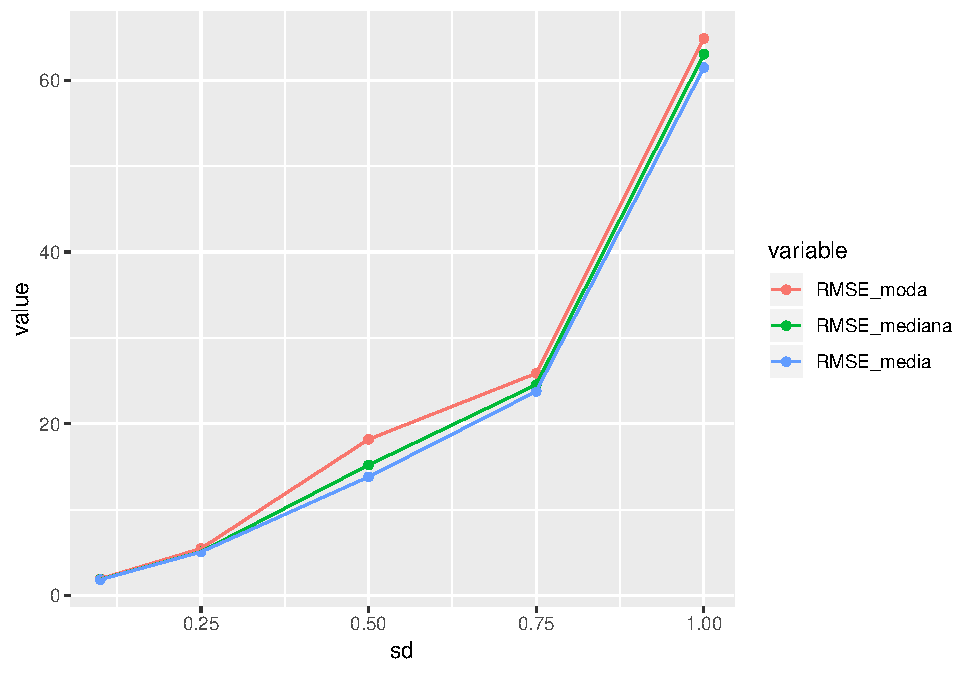
\includegraphics{Impacto_sigma_files/figure-latex/unnamed-chunk-45-1.pdf}

\section{SIMULAÇÕES DE MONTE CARLO}\label{simulacoes-de-monte-carlo}

\begin{Shaded}
\begin{Highlighting}[]
\KeywordTok{set.seed}\NormalTok{(}\DecValTok{1}\NormalTok{)}
\NormalTok{x <-}\StringTok{ }\KeywordTok{seq}\NormalTok{(}\DecValTok{1}\NormalTok{, }\DecValTok{100}\NormalTok{, }\FloatTok{0.5}\NormalTok{)}
\NormalTok{sd <-}\StringTok{ }\KeywordTok{seq}\NormalTok{(}\FloatTok{0.1}\NormalTok{, }\FloatTok{1.5}\NormalTok{, .}\DecValTok{1}\NormalTok{)}
\NormalTok{n <-}\StringTok{ }\DecValTok{500}
\NormalTok{rmse <-}\StringTok{ }\OtherTok{NULL}
\ControlFlowTok{for}\NormalTok{ (i }\ControlFlowTok{in} \KeywordTok{seq_along}\NormalTok{(sd)) \{}
\NormalTok{  moda <-}\StringTok{ }\OtherTok{NULL}
\NormalTok{  mediana <-}\StringTok{ }\OtherTok{NULL}
\NormalTok{  media <-}\StringTok{ }\OtherTok{NULL}
  \ControlFlowTok{for}\NormalTok{ (j }\ControlFlowTok{in} \DecValTok{1}\OperatorTok{:}\NormalTok{n)\{}
\NormalTok{    y <-}\StringTok{ }\KeywordTok{exp}\NormalTok{(x}\OperatorTok{/}\DecValTok{25} \OperatorTok{+}\StringTok{ }\KeywordTok{rnorm}\NormalTok{(}\DecValTok{199}\NormalTok{, }\DataTypeTok{sd =}\NormalTok{ sd[[i]])) }
\NormalTok{    id <-}\StringTok{ }\KeywordTok{sample}\NormalTok{(}\DecValTok{1}\OperatorTok{:}\DecValTok{199}\NormalTok{, }\DecValTok{139}\NormalTok{)}
\NormalTok{    y_train <-}\StringTok{ }\NormalTok{y[id]}
\NormalTok{    y_test <-}\StringTok{  }\NormalTok{y[}\OperatorTok{-}\NormalTok{id]}
\NormalTok{    x_train <-}\StringTok{ }\NormalTok{x[id]}
\NormalTok{    fit <-}\StringTok{ }\KeywordTok{lm}\NormalTok{(}\KeywordTok{log}\NormalTok{(y_train) }\OperatorTok{~}\StringTok{ }\NormalTok{x_train)}
\NormalTok{    s <-}\StringTok{ }\KeywordTok{summary}\NormalTok{(fit)}
\NormalTok{    p <-}\StringTok{ }\KeywordTok{predict}\NormalTok{(fit, }\DataTypeTok{newdata =} \KeywordTok{data.frame}\NormalTok{(}\DataTypeTok{x_train =}\NormalTok{ x[}\OperatorTok{-}\NormalTok{id]))}
\NormalTok{    p_moda <-}\StringTok{ }\KeywordTok{exp}\NormalTok{(p }\OperatorTok{-}\StringTok{ }\NormalTok{s}\OperatorTok{$}\NormalTok{sigma}\OperatorTok{^}\DecValTok{2}\NormalTok{)}
\NormalTok{    p_mediana <-}\StringTok{ }\KeywordTok{exp}\NormalTok{(p)}
\NormalTok{    p_media <-}\StringTok{ }\KeywordTok{exp}\NormalTok{(p }\OperatorTok{+}\StringTok{ }\NormalTok{s}\OperatorTok{$}\NormalTok{sigma}\OperatorTok{^}\DecValTok{2}\OperatorTok{/}\DecValTok{2}\NormalTok{)}
\NormalTok{    moda[[j]] <-}\StringTok{ }\KeywordTok{sqrt}\NormalTok{(}\KeywordTok{mean}\NormalTok{((p_moda }\OperatorTok{-}\StringTok{ }\NormalTok{y_test)}\OperatorTok{^}\DecValTok{2}\NormalTok{))}
\NormalTok{    mediana[[j]] <-}\StringTok{ }\KeywordTok{sqrt}\NormalTok{(}\KeywordTok{mean}\NormalTok{((p_mediana }\OperatorTok{-}\StringTok{ }\NormalTok{y_test)}\OperatorTok{^}\DecValTok{2}\NormalTok{))}
\NormalTok{    media[[j]] <-}\StringTok{ }\KeywordTok{sqrt}\NormalTok{(}\KeywordTok{mean}\NormalTok{((p_media }\OperatorTok{-}\StringTok{ }\NormalTok{y_test)}\OperatorTok{^}\DecValTok{2}\NormalTok{))  }
\NormalTok{  \}}
\NormalTok{  rmse[[i]] <-}\StringTok{ }\KeywordTok{data.frame}\NormalTok{(}\DataTypeTok{sd =}\NormalTok{ sd[[i]], moda, mediana, media)}
\NormalTok{\}}
\NormalTok{rmse <-}\StringTok{ }\KeywordTok{do.call}\NormalTok{(rbind, rmse)}
\NormalTok{rmse }\OperatorTok\StringTok{ }
\StringTok{  }\KeywordTok{rowwise}\NormalTok{() }\OperatorTok\StringTok{ }
\StringTok{  }\KeywordTok{mutate}\NormalTok{(}\DataTypeTok{Min =} \KeywordTok{which.min}\NormalTok{(}\KeywordTok{c}\NormalTok{(moda, mediana, media)))}
\end{Highlighting}
\end{Shaded}

\begin{Shaded}
\begin{Highlighting}[]
\NormalTok{medias <-}\StringTok{ }\NormalTok{rmse }\OperatorTok
\StringTok{  }\KeywordTok{group_by}\NormalTok{(sd) }\OperatorTok
\StringTok{  }\KeywordTok{summarise}\NormalTok{(}\DataTypeTok{Moda =} \KeywordTok{mean}\NormalTok{(moda), }
            \DataTypeTok{Mediana =} \KeywordTok{mean}\NormalTok{(mediana), }
            \DataTypeTok{Media =} \KeywordTok{mean}\NormalTok{(media))}
\end{Highlighting}
\end{Shaded}

\begin{verbatim}
## Warning: Grouping rowwise data frame strips rowwise nature
\end{verbatim}

\begin{Shaded}
\begin{Highlighting}[]
\NormalTok{n <-}\StringTok{ }\NormalTok{rmse }\OperatorTok
\StringTok{  }\KeywordTok{group_by}\NormalTok{(sd, Min) }\OperatorTok
\StringTok{  }\KeywordTok{summarise}\NormalTok{(}\KeywordTok{n}\NormalTok{())}
\end{Highlighting}
\end{Shaded}

\begin{verbatim}
## Warning: Grouping rowwise data frame strips rowwise nature
\end{verbatim}

\begin{Shaded}
\begin{Highlighting}[]
\NormalTok{medias <-}\StringTok{ }\KeywordTok{melt}\NormalTok{(medias, }\DataTypeTok{id =} \StringTok{"sd"}\NormalTok{)}
\KeywordTok{ggplot}\NormalTok{(medias, }\KeywordTok{aes}\NormalTok{(}\DataTypeTok{x =}\NormalTok{ sd, }\DataTypeTok{y =}\NormalTok{ value, }\DataTypeTok{color =}\NormalTok{ variable)) }\OperatorTok{+}\StringTok{ }
\StringTok{  }\KeywordTok{geom_point}\NormalTok{() }\OperatorTok{+}\StringTok{ }
\StringTok{  }\KeywordTok{geom_line}\NormalTok{()}
\end{Highlighting}
\end{Shaded}

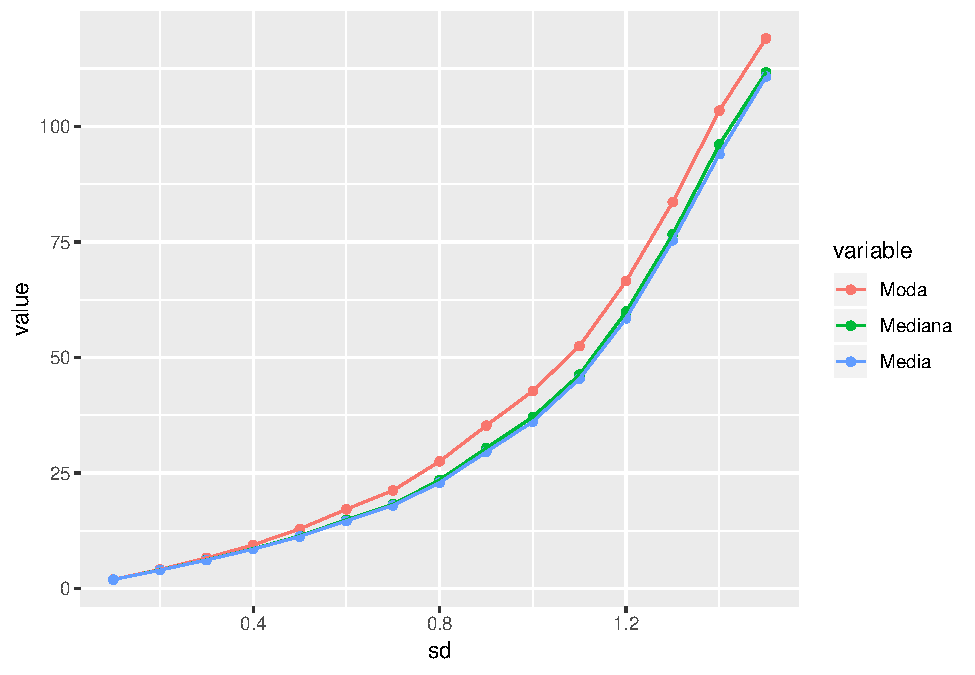
\includegraphics{Impacto_sigma_files/figure-latex/unnamed-chunk-48-1.pdf}

\begin{Shaded}
\begin{Highlighting}[]
\KeywordTok{ggplot}\NormalTok{(n, }\KeywordTok{aes}\NormalTok{(}\DataTypeTok{x =}\NormalTok{ sd, }\DataTypeTok{y =} \StringTok{`}\DataTypeTok{n()}\StringTok{`}\NormalTok{, }
              \DataTypeTok{color =} \KeywordTok{factor}\NormalTok{(Min, }
                             \DataTypeTok{levels =} \KeywordTok{c}\NormalTok{(}\DecValTok{1}\NormalTok{, }\DecValTok{2}\NormalTok{, }\DecValTok{3}\NormalTok{), }
                             \DataTypeTok{labels =} \KeywordTok{c}\NormalTok{(}\StringTok{"moda"}\NormalTok{, }\StringTok{"mediana"}\NormalTok{, }\StringTok{"media"}\NormalTok{)))) }\OperatorTok{+}\StringTok{ }
\StringTok{  }\KeywordTok{geom_point}\NormalTok{() }\OperatorTok{+}\StringTok{ }
\StringTok{  }\KeywordTok{geom_line}\NormalTok{() }\OperatorTok{+}\StringTok{ }
\StringTok{  }\KeywordTok{guides}\NormalTok{(}\DataTypeTok{color=}\KeywordTok{guide_legend}\NormalTok{(}\DataTypeTok{title=}\StringTok{"Estimativa"}\NormalTok{))}
\end{Highlighting}
\end{Shaded}

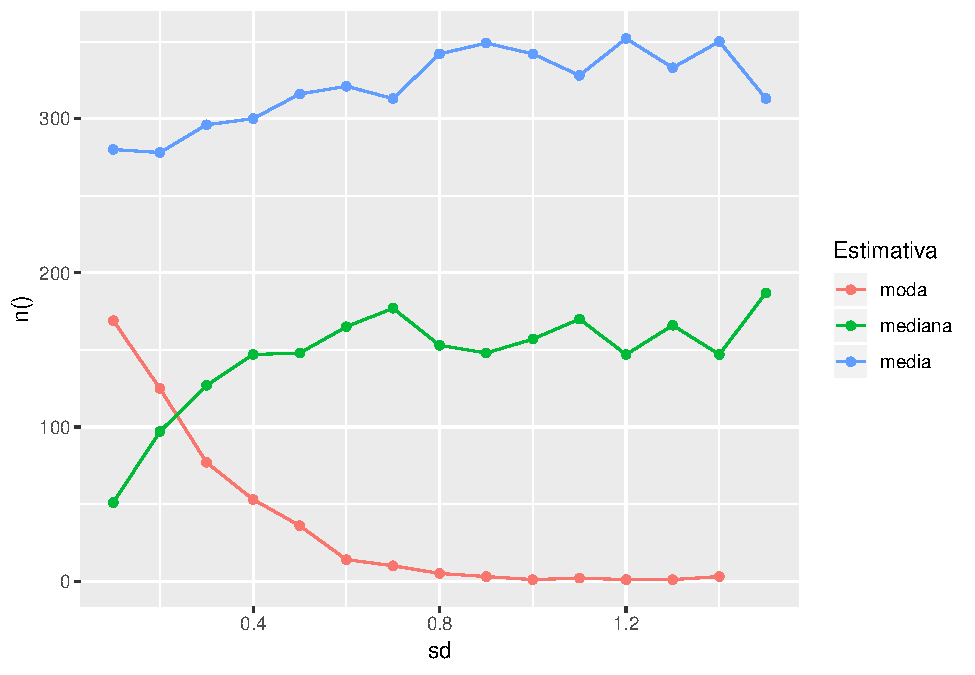
\includegraphics{Impacto_sigma_files/figure-latex/unnamed-chunk-49-1.pdf}

\section{REGRESSÃO À MEDIANA}\label{regressao-a-mediana}

\section{VALIDAÇÃO CRUZADA}\label{validacao-cruzada-1}

\subsection{Modelo 1}\label{modelo-1-2}

\begin{Shaded}
\begin{Highlighting}[]
\NormalTok{fit <-}\StringTok{ }\KeywordTok{rq}\NormalTok{(}\KeywordTok{log}\NormalTok{(y_train) }\OperatorTok{~}\StringTok{ }\NormalTok{x_train)}
\NormalTok{s <-}\StringTok{ }\KeywordTok{summary}\NormalTok{(fit)}
\NormalTok{p <-}\StringTok{ }\KeywordTok{predict}\NormalTok{(fit, }\DataTypeTok{newdata =} \KeywordTok{data.frame}\NormalTok{(}\DataTypeTok{x_train =}\NormalTok{ x[}\OperatorTok{-}\NormalTok{id]))}
\NormalTok{p_mediana <-}\StringTok{ }\KeywordTok{exp}\NormalTok{(p)}
\NormalTok{(mape <-}\StringTok{ }\KeywordTok{mean}\NormalTok{(}\KeywordTok{abs}\NormalTok{(p_mediana }\OperatorTok{-}\StringTok{ }\NormalTok{y_test)))}
\end{Highlighting}
\end{Shaded}

\begin{verbatim}
## [1] 14.51783
\end{verbatim}

\subsection{Modelo 2}\label{modelo-2-2}

\begin{Shaded}
\begin{Highlighting}[]
\NormalTok{fit1 <-}\StringTok{ }\KeywordTok{rq}\NormalTok{(}\KeywordTok{log}\NormalTok{(y1_train) }\OperatorTok{~}\StringTok{ }\NormalTok{x_train)}
\NormalTok{s1 <-}\StringTok{ }\KeywordTok{summary}\NormalTok{(fit1)}
\NormalTok{p1 <-}\StringTok{ }\KeywordTok{predict}\NormalTok{(fit1, }\DataTypeTok{newdata =} \KeywordTok{data.frame}\NormalTok{(}\DataTypeTok{x_train =}\NormalTok{ x[}\OperatorTok{-}\NormalTok{id]))}
\NormalTok{p1_mediana <-}\StringTok{ }\KeywordTok{exp}\NormalTok{(p1)}
\NormalTok{(mape1 <-}\StringTok{ }\KeywordTok{mean}\NormalTok{(}\KeywordTok{abs}\NormalTok{(p1_mediana }\OperatorTok{-}\StringTok{ }\NormalTok{y1_test)))}
\end{Highlighting}
\end{Shaded}

\begin{verbatim}
## [1] 12.81536
\end{verbatim}

\subsection{Modelo 3}\label{modelo-3-2}

\begin{Shaded}
\begin{Highlighting}[]
\NormalTok{fit2 <-}\StringTok{ }\KeywordTok{rq}\NormalTok{(}\KeywordTok{log}\NormalTok{(y2_train) }\OperatorTok{~}\StringTok{ }\NormalTok{x_train)}
\NormalTok{s2 <-}\StringTok{ }\KeywordTok{summary}\NormalTok{(fit2)}
\NormalTok{p2 <-}\StringTok{ }\KeywordTok{predict}\NormalTok{(fit2, }\DataTypeTok{newdata =} \KeywordTok{data.frame}\NormalTok{(}\DataTypeTok{x_train =}\NormalTok{ x[}\OperatorTok{-}\NormalTok{id]))}
\NormalTok{p2_mediana <-}\StringTok{ }\KeywordTok{exp}\NormalTok{(p2)}
\NormalTok{(mape2 <-}\StringTok{ }\KeywordTok{mean}\NormalTok{(}\KeywordTok{abs}\NormalTok{(p2_mediana }\OperatorTok{-}\StringTok{ }\NormalTok{y2_test)))}
\end{Highlighting}
\end{Shaded}

\begin{verbatim}
## [1] 14.11574
\end{verbatim}

\subsection{Modelo 4}\label{modelo-4-2}

\begin{Shaded}
\begin{Highlighting}[]
\NormalTok{fit3 <-}\StringTok{ }\KeywordTok{rq}\NormalTok{(}\KeywordTok{log}\NormalTok{(y3_train) }\OperatorTok{~}\StringTok{ }\NormalTok{x_train)}
\NormalTok{s3 <-}\StringTok{ }\KeywordTok{summary}\NormalTok{(fit3)}
\NormalTok{p <-}\StringTok{ }\KeywordTok{predict}\NormalTok{(fit3, }\DataTypeTok{newdata =} \KeywordTok{data.frame}\NormalTok{(}\DataTypeTok{x_train =}\NormalTok{ x[}\OperatorTok{-}\NormalTok{id]))}
\NormalTok{p3_mediana <-}\StringTok{ }\KeywordTok{exp}\NormalTok{(p3)}
\NormalTok{(mape3 <-}\StringTok{ }\KeywordTok{mean}\NormalTok{(}\KeywordTok{abs}\NormalTok{(p3_mediana }\OperatorTok{-}\StringTok{ }\NormalTok{y3_test)))}
\end{Highlighting}
\end{Shaded}

\begin{verbatim}
## [1] 13.29267
\end{verbatim}

\subsection{Modelo 5}\label{modelo-5-1}

\begin{Shaded}
\begin{Highlighting}[]
\NormalTok{fit4 <-}\StringTok{ }\KeywordTok{rq}\NormalTok{(}\KeywordTok{log}\NormalTok{(y4_train) }\OperatorTok{~}\StringTok{ }\NormalTok{x_train)}
\NormalTok{s4 <-}\StringTok{ }\KeywordTok{summary}\NormalTok{(fit4)}
\NormalTok{p <-}\StringTok{ }\KeywordTok{predict}\NormalTok{(fit4, }\DataTypeTok{newdata =} \KeywordTok{data.frame}\NormalTok{(}\DataTypeTok{x_train =}\NormalTok{ x[}\OperatorTok{-}\NormalTok{id]))}
\NormalTok{p4_mediana <-}\StringTok{ }\KeywordTok{exp}\NormalTok{(p4)}
\NormalTok{(mape4 <-}\StringTok{ }\KeywordTok{mean}\NormalTok{(}\KeywordTok{abs}\NormalTok{(p4_mediana }\OperatorTok{-}\StringTok{ }\NormalTok{y4_test)))}
\end{Highlighting}
\end{Shaded}

\begin{verbatim}
## [1] 28.11301
\end{verbatim}

\begin{Shaded}
\begin{Highlighting}[]
\NormalTok{df <-}\StringTok{ }\KeywordTok{data.frame}\NormalTok{(}\DataTypeTok{sd =} \KeywordTok{c}\NormalTok{(}\FloatTok{0.1}\NormalTok{, }\FloatTok{0.25}\NormalTok{, }\FloatTok{0.5}\NormalTok{, }\FloatTok{0.75}\NormalTok{, }\DecValTok{1}\NormalTok{),}
                 \DataTypeTok{MAPE =} \KeywordTok{c}\NormalTok{(mape, mape1, mape2, mape3, mape4))}
\NormalTok{df <-}\StringTok{ }\KeywordTok{melt}\NormalTok{(df, }\DataTypeTok{id =} \StringTok{"sd"}\NormalTok{)}
\end{Highlighting}
\end{Shaded}

\begin{Shaded}
\begin{Highlighting}[]
\KeywordTok{ggplot}\NormalTok{(df, }\KeywordTok{aes}\NormalTok{(}\DataTypeTok{x =}\NormalTok{ sd, }\DataTypeTok{y =}\NormalTok{ value, }\DataTypeTok{color =}\NormalTok{ variable)) }\OperatorTok{+}\StringTok{ }
\StringTok{  }\KeywordTok{geom_point}\NormalTok{() }\OperatorTok{+}\StringTok{ }\KeywordTok{geom_line}\NormalTok{()}
\end{Highlighting}
\end{Shaded}

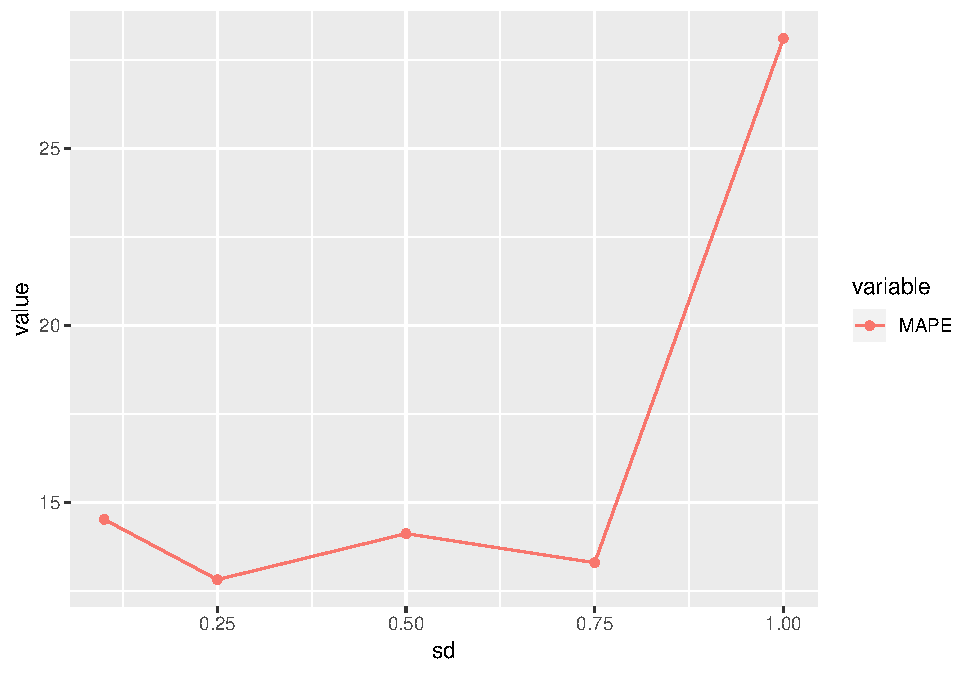
\includegraphics{Impacto_sigma_files/figure-latex/unnamed-chunk-56-1.pdf}

\section*{REFERÊNCIAS}\label{referencias}
\addcontentsline{toc}{section}{REFERÊNCIAS}

\hypertarget{refs}{}
\hypertarget{ref-hochheim}{}
HOCHHEIM, N. \textbf{Engenharia de avaliações - módulo básico}.
Florianópolis: IBAPE - SC, 2015.

\hypertarget{ref-limpert}{}
LIMPERT, E.; A. STAHEL, W.; ABBT, M. Log-normal distributions across the
sciences: Keys and clues., v. 51, p. 341, 2001.


\end{document}
